\section{Redundant file characterization}
\label{sec:redundant_files}
\nancomment{1. high repeat cnt type examples
			2. use case for each type
			3. analyze the others cluster, if have time}

\begin{figure*}
	\centering
	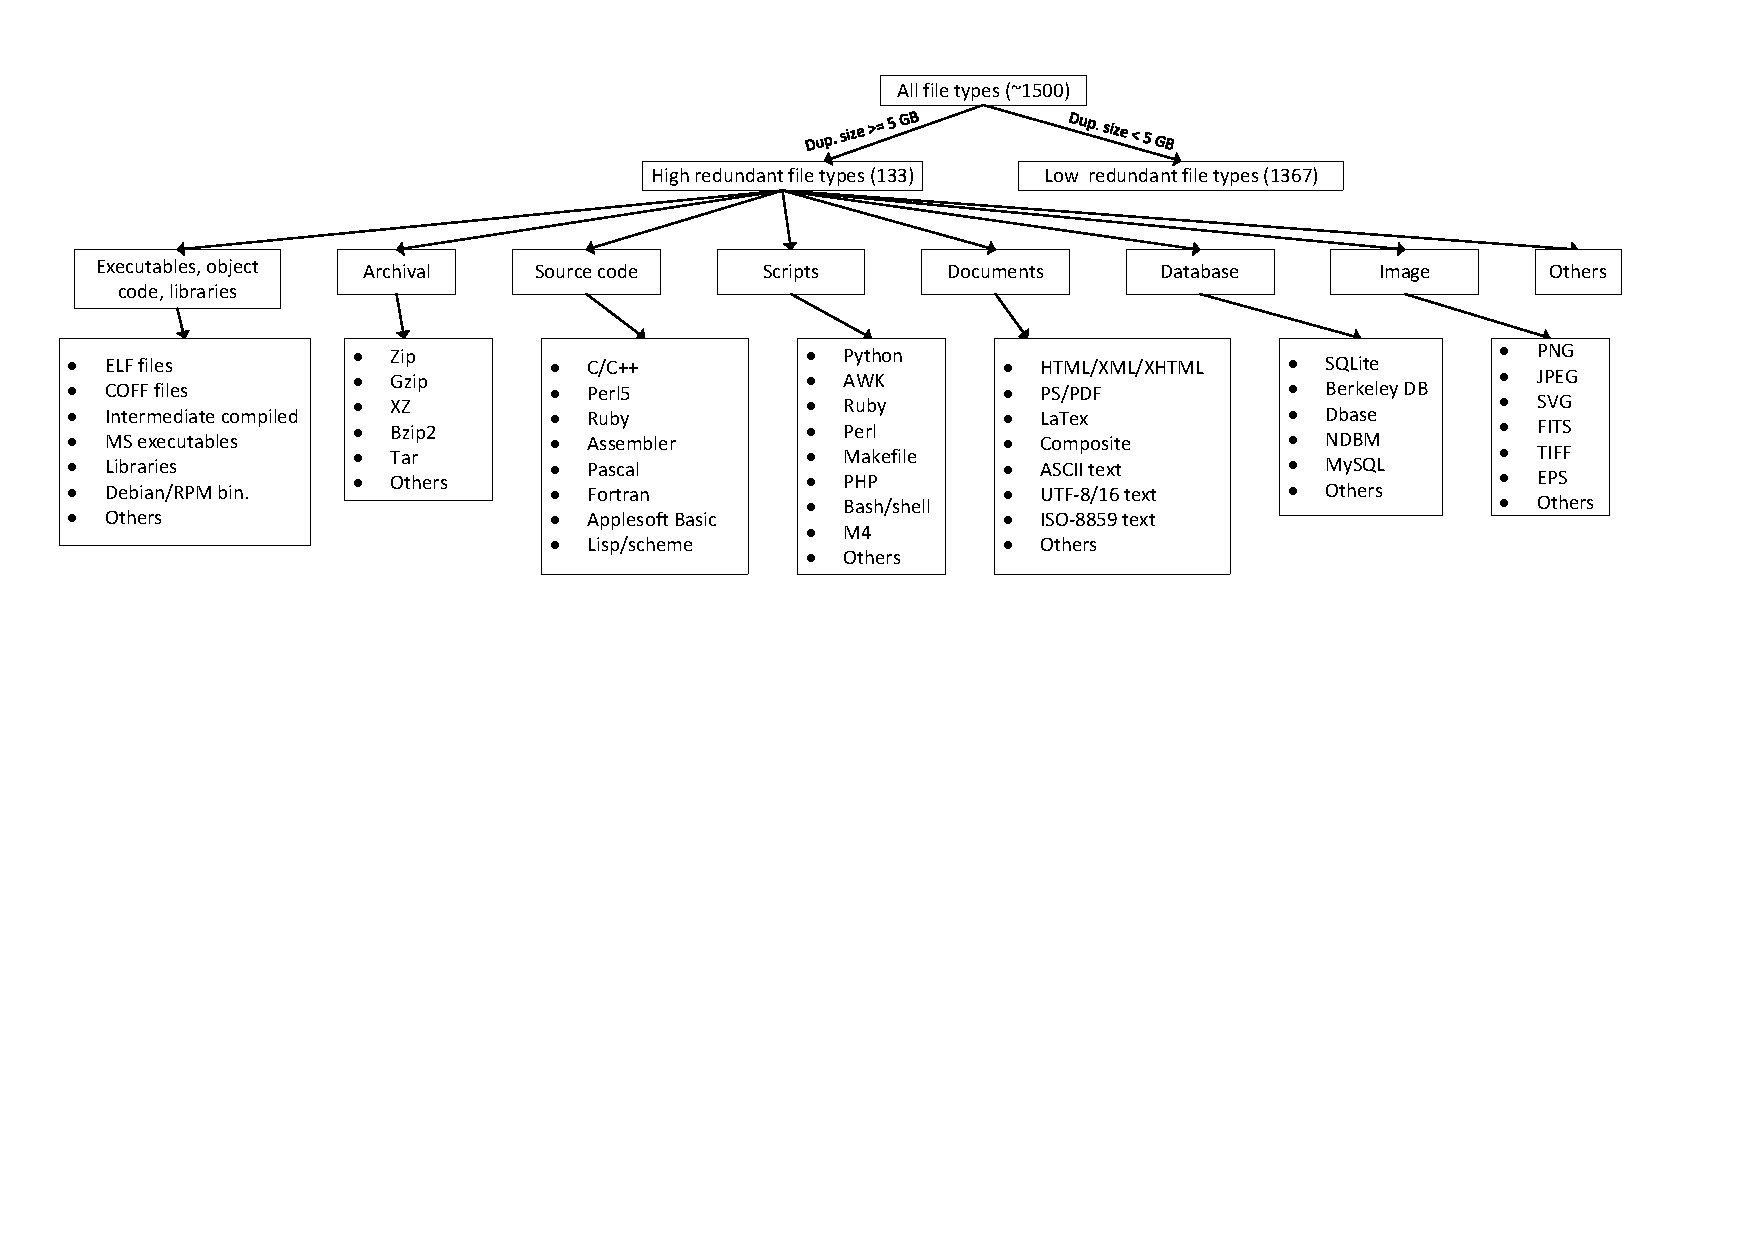
\includegraphics[width=1\textwidth]{graphs/graph-types-hierarchy}
	\caption{Taxonomy of file types.
	}
	\label{fig:file-type-hierarchy}
\end{figure*}

In this section, we present our redundant file characterization on file repeat count, file size, and file types. 
Based on this characterization, we create three-level classification hierarchy as shown in Figure~\ref{fig:file-type-hierarchy}.
At the highest level, we created two categories: \textit{High redundant file types and low redundant file types} based on the total redundant file size for each type. 
Totally, we got around 1,500 types after analyzing our whole dataset. 
We found that only 133 file types's total redundant file sizes are greater than 5 GB, which take up to 98.4\% files with 166.8 TB totally. We put these 133 file types into high redundant file type group and the remaining files into low redundant file types. Our further classification expands on the 98.4\% common redundant file types. 

%are common file types that consists of a largest number of redundant files with large storage space consumed, such as xxx and xxx. 
%Only xxxx\% files are non-common file types that only contains a small number of redundant files with less storage space, such as xxxx and xxxx. 
 
At the second level of the hierarchy, we clustered high redundant file types based on the \textit{major file format, usage or platform} involved by each file type. We identified redundant files' types relevant to \textit{EOF (executable, object code, and libraries), source code, scripts, documents, archival, images, databases, and others}.

At the third level, we present the specific redundant file types which take a large percentage of redundant files or storage space.
% or further classify the redundant files based on involved by each file type. 
%We selected the file types which take largest storage space.  
Based on the second-and third-level classification, we investigated the following two research questions: (1) What are the common redundant files?
(2) Why there are so many redundant files? and present our investigation results.

\begin{figure}
	\centering
	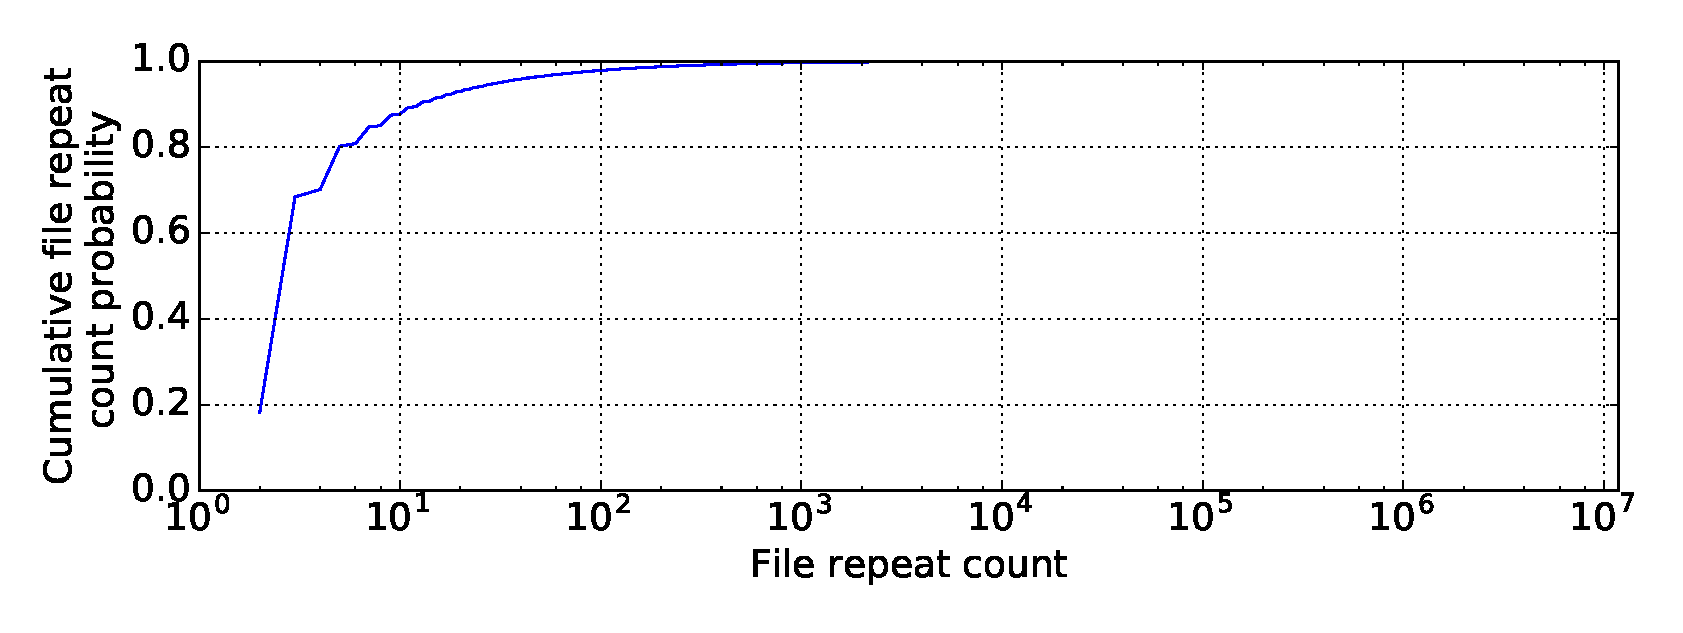
\includegraphics[width=0.5\textwidth]{graphs/File_repeat_count.eps}
	\caption{File repeat count distribution.
	}
	\label{fig:file-repeat-cnt}
\end{figure}

Figure~\ref{fig:file-repeat-cnt} shows the cumulative and probability distribution of file repeat count. 
Most files have a small repeat count. For instance, almost 90\% of files have equal or less than 10 copies. Around 50\% of files have 4 copies.
The file that has the maximum repeat count is empty file, which means that many users creates empty files and stored in their images.
%\subsection{File repeat count}
%\subsection{File size}

\begin{figure}
	\centering
	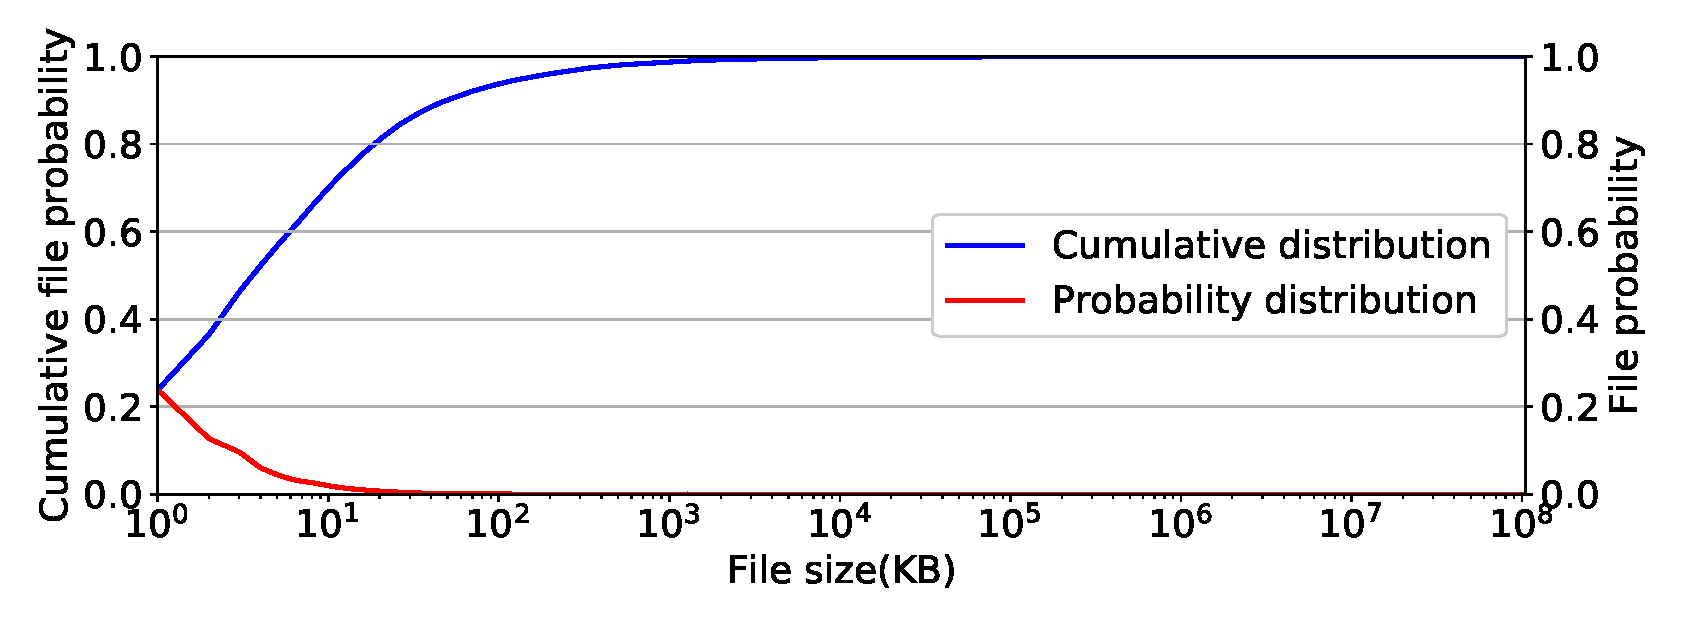
\includegraphics[width=0.5\textwidth]{graphs/File_size-KB.eps}
	\caption{File size distribution.
	}
	\label{fig:file-size}
\end{figure}

Figure~\ref{fig:file-size} shows the cumulative and probability distribution of file size of unique dataset after we remove the redundant files.
Most files are smaller files. For example, 91\% files'sizes are equal or less than 100KB. 
Around 22\% of files are less than 1 KB.
 

\subsection{Overview of high redundant file types}

\paragraph{Finding 1: 13.38\% and 10.23\% of redundant files are source codes and EOL files, which take up over 3.66\% (5.3 TB) and 36.85\% (52.9 TB) of redundant storage space, indicating that users are more prone to replicate source codes and create identical big EOF files, while 43.15\% and 8.53\% of redundant files are documents and archival files, which account for 14.54\% (20.87 TB) and 22.93\% (32.9 TB) of redundant storage space, indicating users replicates more documents and archival files compare to other clusters}

%Some data is inherently more prone to duplicates than others.
Figure~\ref{fig:file-types} presents redundant data vs. unique data for each clusters. 
Document cluster has the largest number of redundant files (43.15\%), indicating that users replicate more documents than other clusters. While the redundant document files only consume 14.54\% (20.87 TB) of storage space, indicating that the size of redundant document files are small (10.2 KB on average). In comparison, 13.38\% and 10.23\% of files are EOL files and source codes, which take up over 3.66\% (5.3 TB) and 36.85\% (52.9 TB) of redundant storage space, indicating that users replicate source codes and create big identical EOF files (108.6 KB on average).

Archival files and scripts have almost similarly number of redundant files, 8.53\% for archival and 8.69\% for scripts. However, archival cluster consumes more storage space than that of scripts (32.9 TB for archival and 3.9 TB for scripts) since archival file size (81 KB on avg.) is inherently higher than script size (9.4 KB on avg.).

We found that 4.15\% of redundant files are image files and 0.09\% of redundant files are relevant to database, which takes 2.1 TB and 3.9 GB storage space respectively. There are 10.17\% (21.2 TB) of redundant files in \textit{Other} cluster which mainly contains binary data (9.76), GNU message catalog (3.37 TB), font related type (3.02 TB), git pack files (1.9 TB), etc. 

\begin{figure}
	\centering
	\subfigure[Redundant data vs. unique data in terms of file count.]{\label{fig:file-types-cnt}
		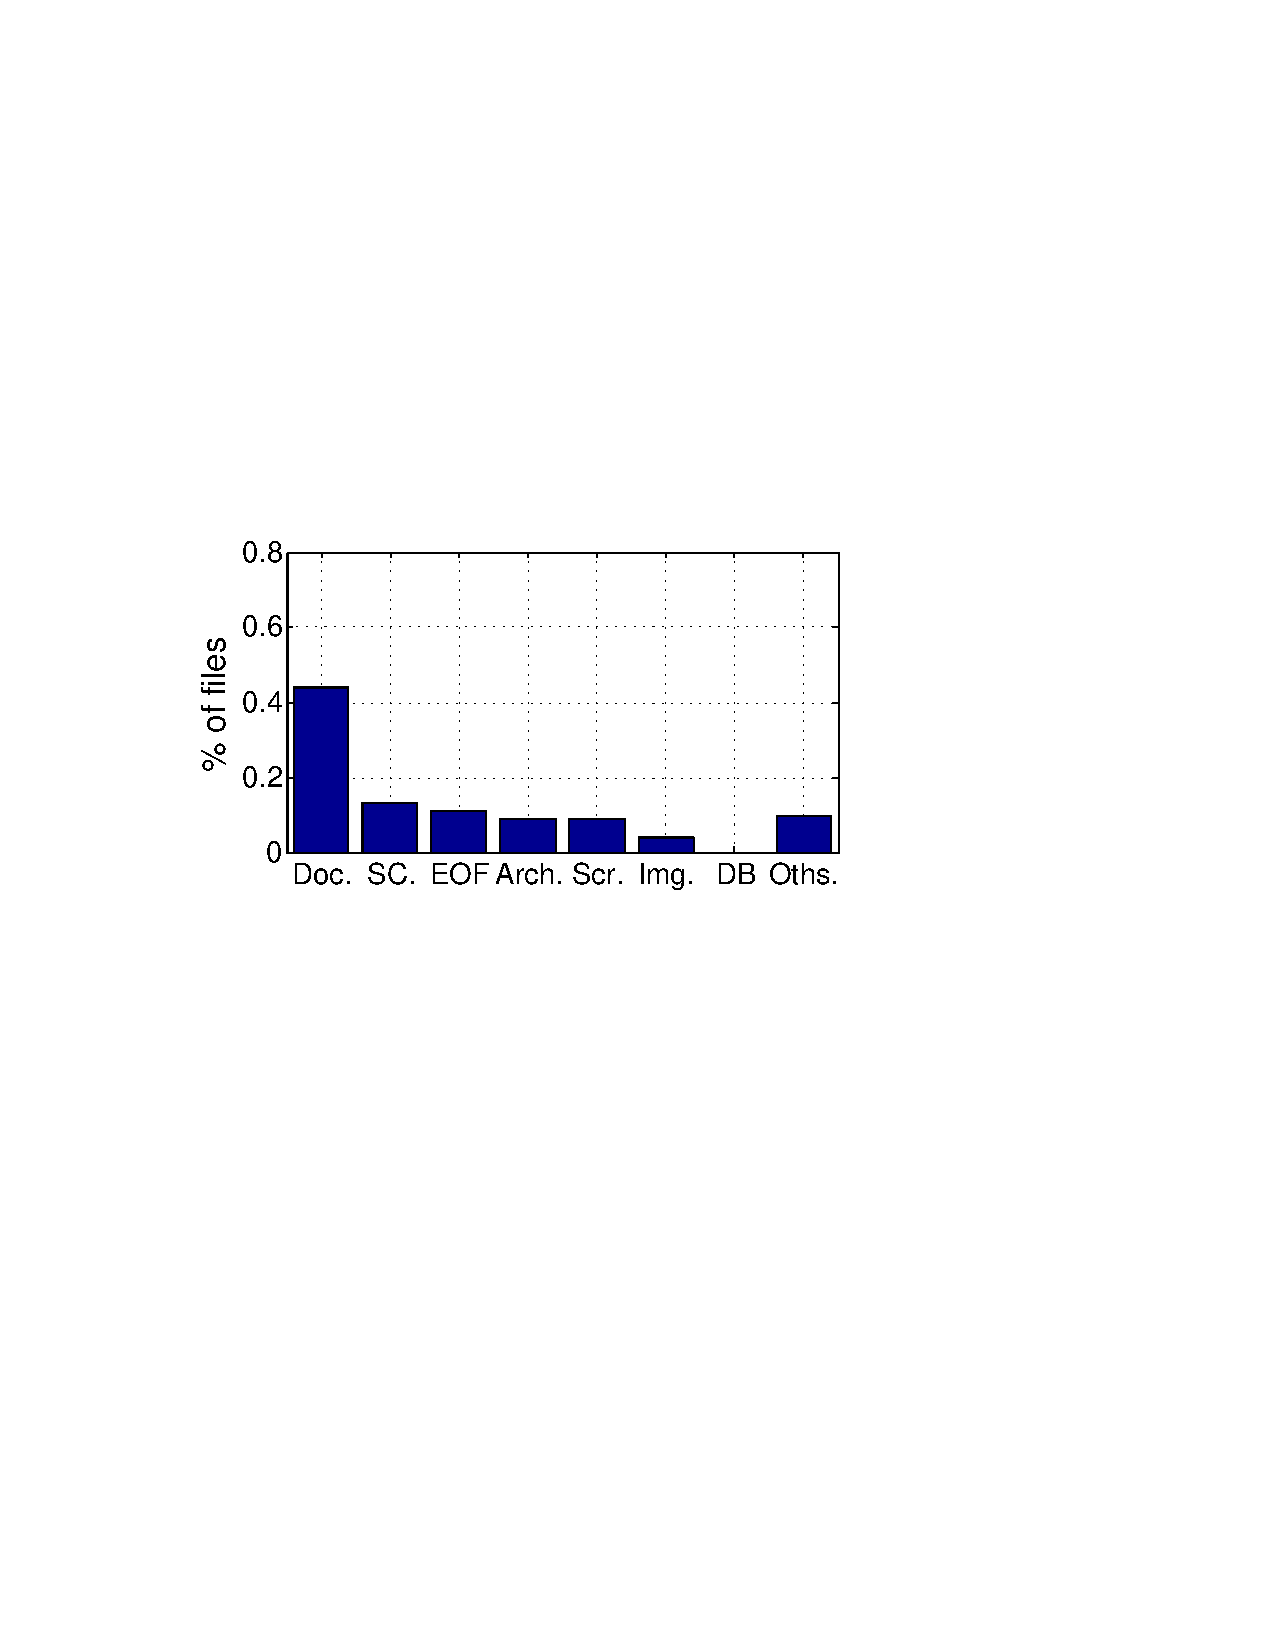
\includegraphics [width=0.4\textwidth]{graphs/type-total-cnt}
	}
	\subfigure[Redundant data vs. unique data in terms of capacity.]{\label{fig:file-types-cap}
		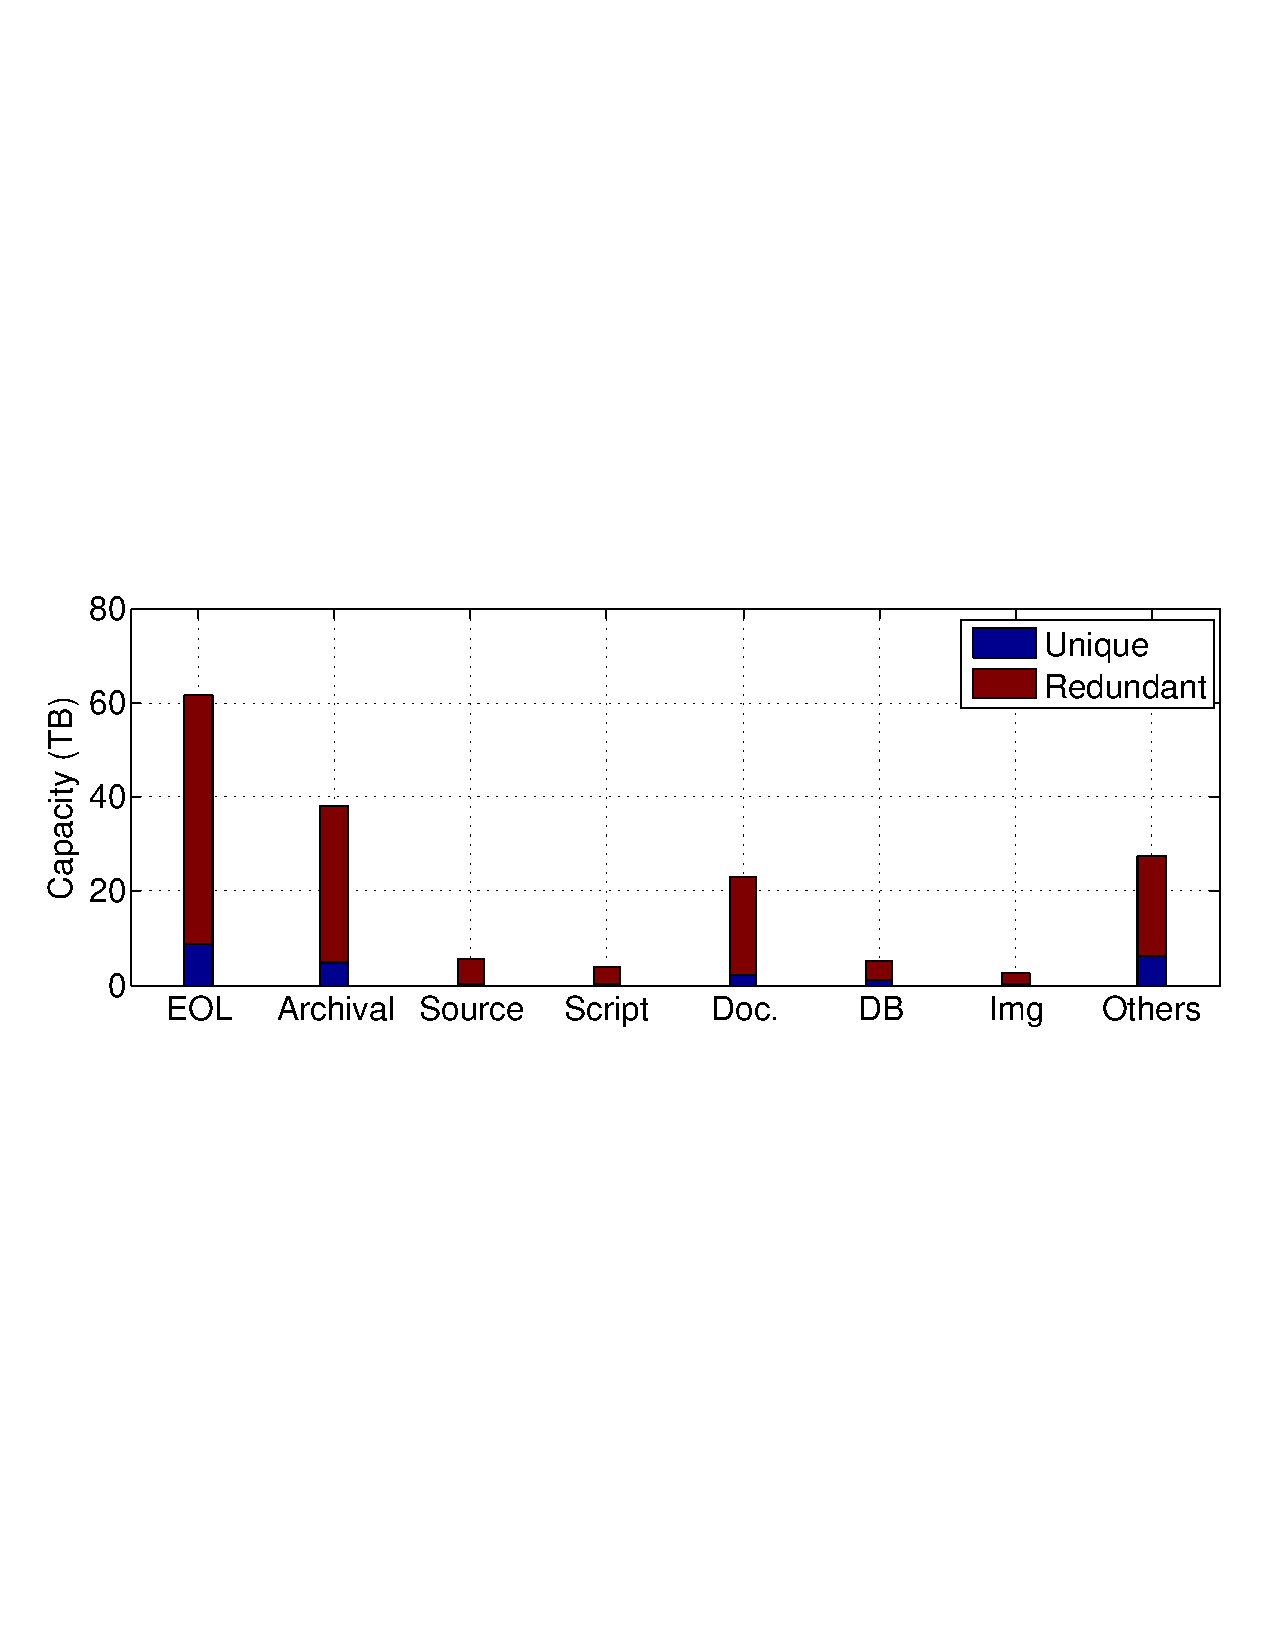
\includegraphics [width=0.4\textwidth]{graphs/type-total-cap}
	}
	\caption{Redundant data vs. unique data for high redundant file types}
	\label{fig:file-types}
\end{figure}

\subsection{EOL files and source codes}

\paragraph{Finding 2: 31.4\% (164,059,690) and 63.7\% (333,261,220) of EOL files are ELF files and intermediate compiled files, which take up over 85.7\% (45.3TB) and 5.3\% (2.8TB) of redundant storage capacity, indicating that users replicate or create more identical ELF files and intermediate compiled files. 64.1\% (213,753,591) of intermediate compiled files are Python byte-compiled files, which take up to 79.4\% (2.2TB) of redundant storage space, indicating that users compiled more Python scripts (similar to Finding 2.)}

As shown in Figure~\ref{fig:type-eol}, intermediate compiled files have the largest number of redundant copies (333,261,220, 63.7\%), which only take up to 5.3\% (2.8TB) of EOL redundant storage space, indicating that users creates more small redundant intermediate compiled files. Among all the intermediate compiled files, python byte-compiled files have the largest number of redundant copies (64.1\%, 213,753,591), which account for 79.4\% (2.2TB) of EOL redundant storage space as shown in Figure~\ref{fig:type-compiled}. 

We found that there are various redundant intermediate compiled files in layers in addition to Python byte-compiled, such as Erlang beam files, Xemacs/emacs compiled files, compiled Java class, Mach-o fat files, Guile object bytecode, and llvm bitcode files. We see that 21.6\% (71,830,155) and 10.12\% (33,740,399) of redundant intermediate compiled files are terminfo compiled and compiled java class files, which consume 76.4 GB and 104.4 GB storage space.   

%ELF files have the largest redundant capacity
%A large executable group is ELF file type, which consists of ELF 64/32-bit LSB relocatable, shared object, executable, core file, processor-specific for x86-64, MIPS,
%ARM, Intel 80386, etc. architectures.
%Another executable group contains VAX COFF executable, PE32/PE32+ executable for Windows, and 386 pure executable, VMS Alpha, etc.
%\% of files are script executable, which contains python, shell, etc.
%\% of files are RPM, Debian bin

\paragraph{Finding 3: 80.2\% (548,507,865) of source codes are C/C++ source, which take up to 79.7\% (4.2TB) of redundant storage space, indicating that users are more prone to duplicate C/C++ codes, which results in more ELF file replicas.}
%The last group contains

\begin{figure}
	\centering
	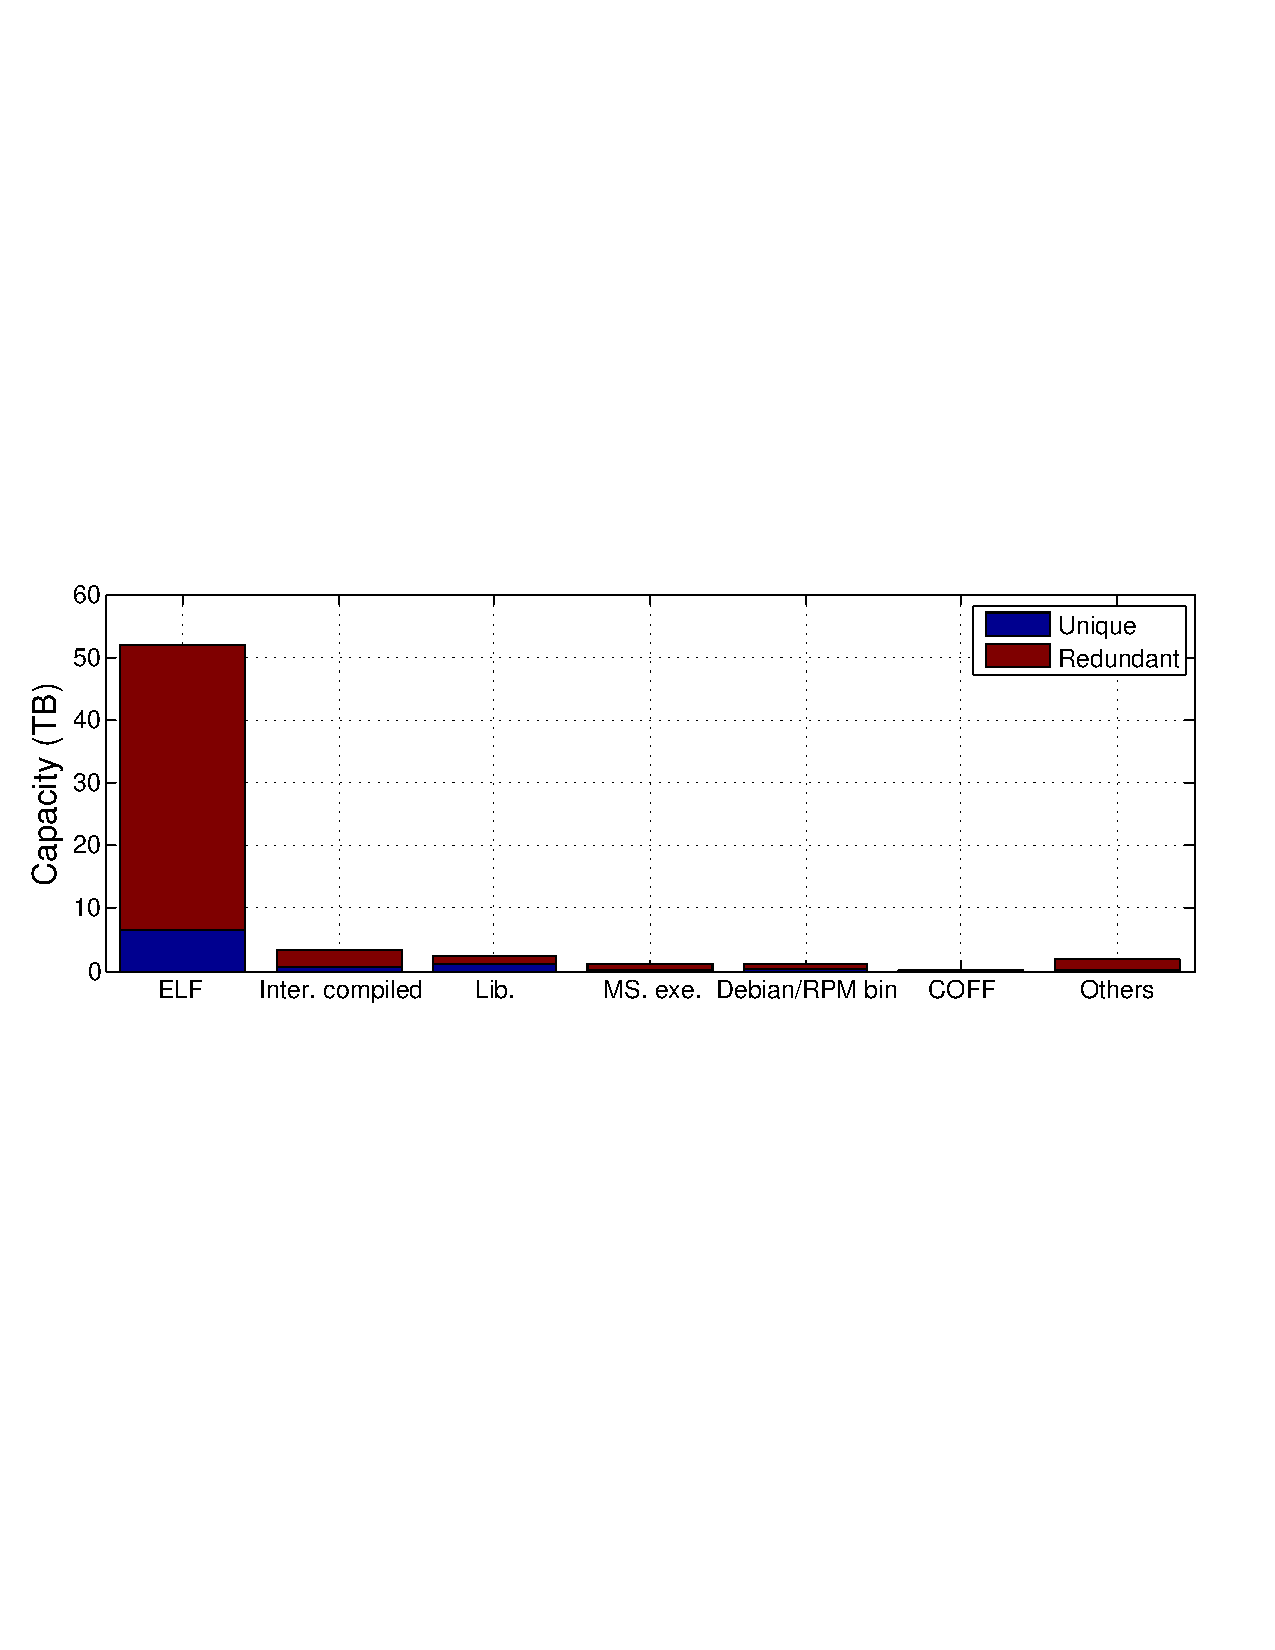
\includegraphics[width=0.5\textwidth]{graphs/type-exec-cap}
	\caption{Redundant data vs. unique data for EOL (Executable, object code, libraries) files.
	}
	\label{fig:type-eol}
\end{figure}

Figure~\ref{fig:type-source} shows the redundant file count and storage capacity distribution for source code. C/C++ source codes have the largest number of redundant files. 80.2\% (548,507,865) of source codes are C/C++ source, which take up to 79.7\% (4.2TB) of redundant storage space, indicating that users are more prone to duplicate C/C++ codes, which results in more ELF file replicas.

We also found other source codes, such as Perl5 module source code (9.5\%), ruby module source code (7.6\%), assembler source code (1.1\%), pascal source (0.7\%), fortran program code (0.01\%), applesoft basic source code, and Lisp/scheme source code (0.17\%).

\begin{figure}
	\centering
	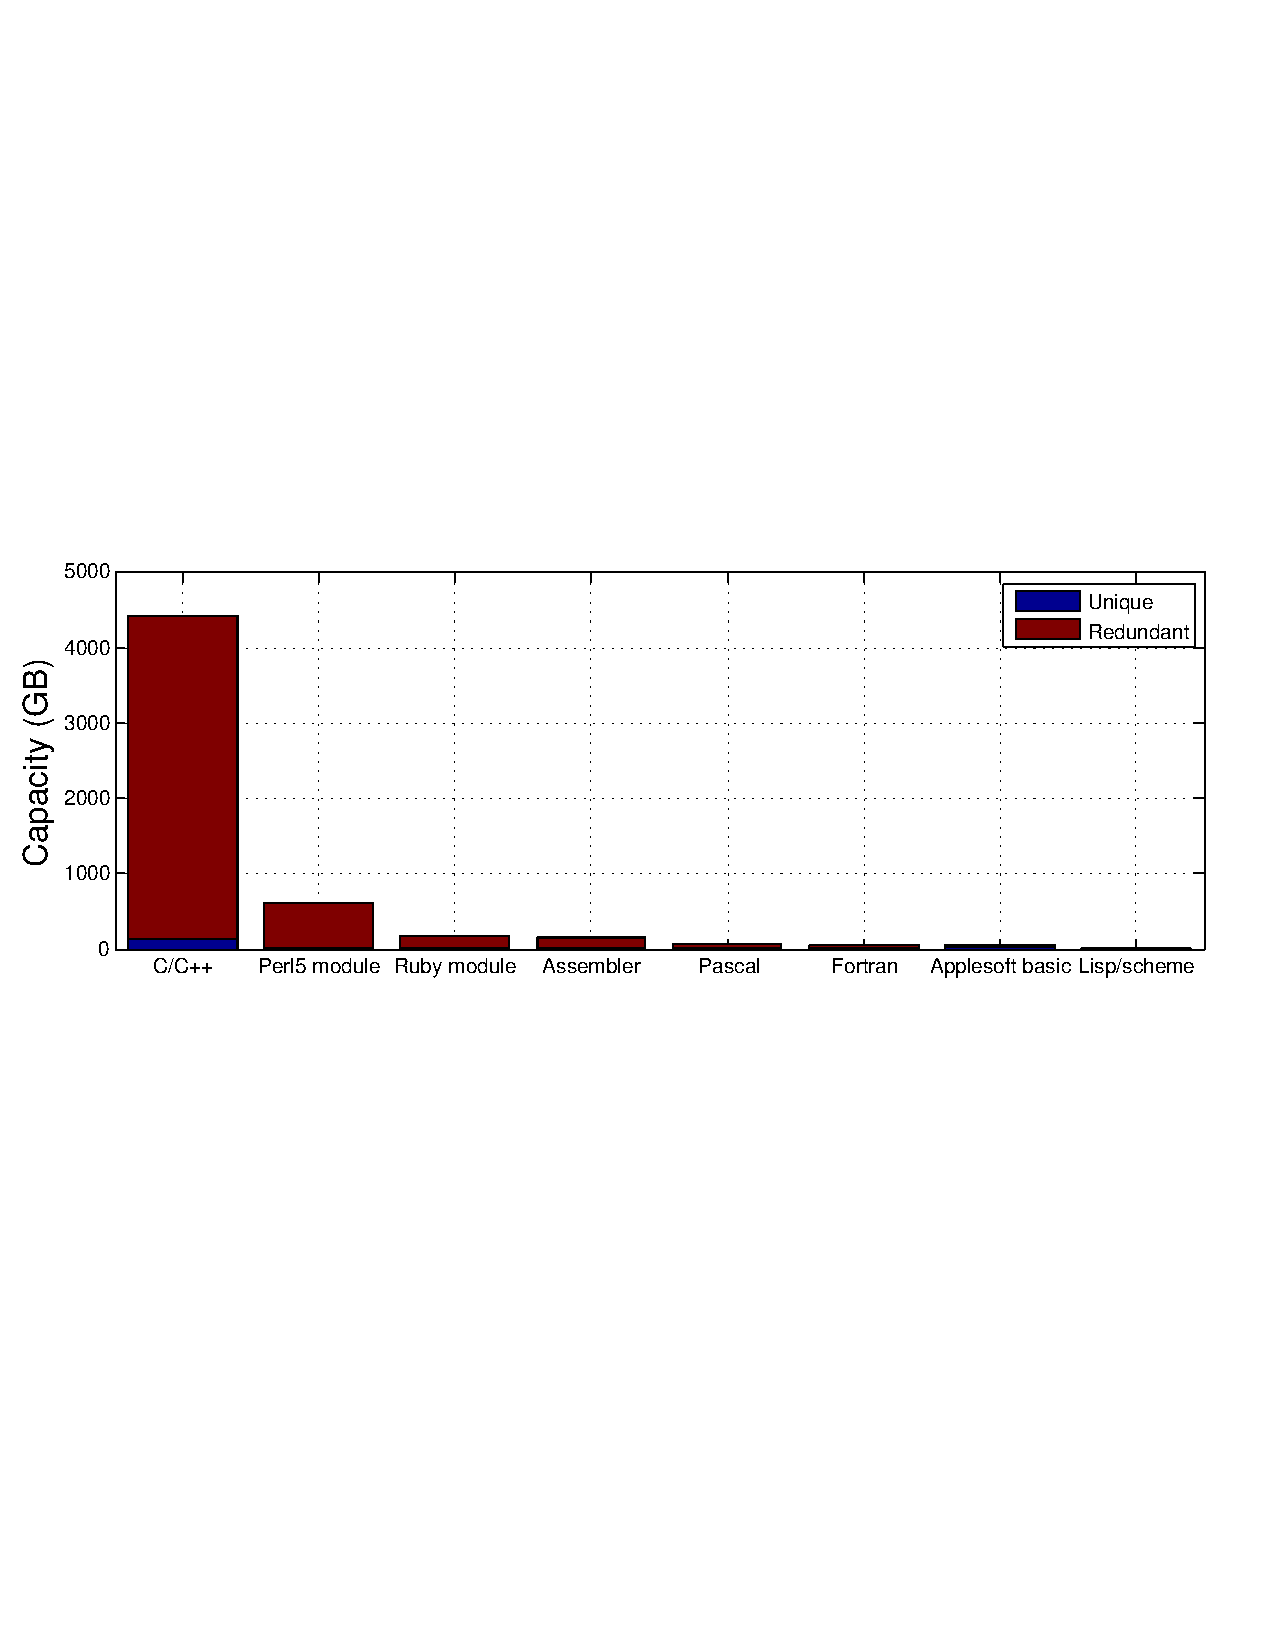
\includegraphics[width=0.5\textwidth]{graphs/type-lang-cap}
	\caption{Redundant data vs. unique data for source code files.
	}
	\label{fig:type-source}
\end{figure}

Figure~\ref{fig:type-lib} shows the redundant library distribution. We see that Gcc precompiled header files have the lowest number of redundant library files (20.3\%), but they take up to 0.93 TB. Almost 86.4\% of redundant library files are Palm libraries, which only take up to 7.2GB space, indicating that gcc compiled header files are much bigger than other libraries.

We also found there are different libraries used in layers, such as netcdf library, Ocaml lib., mach-o lib.

%Figure~\ref{fig-elf}
%\subsection{Lib}
%
%library files contains libtool library file, OCaml native library, MIT scheme, Mach-O library, OCaml library, Palm OS dynamic library data, Microsoft c/c++ library.current ar archive random library, and other library.
%%libtool\|OCaml\|Palm\|MIT\|microsoft\|current ar archive random library\|mach-o\|rpm\|gzip
%\subsection{Source code}

\subsection{Scripts}
\paragraph{Finding 2: 53.6\% (238,353,674) of redundant scripts are Python scripts, which take up over 2.6TB storage space, indicating that users are more prone to replicate Python scripts compare to other scripts}

\begin{figure}
	\centering
	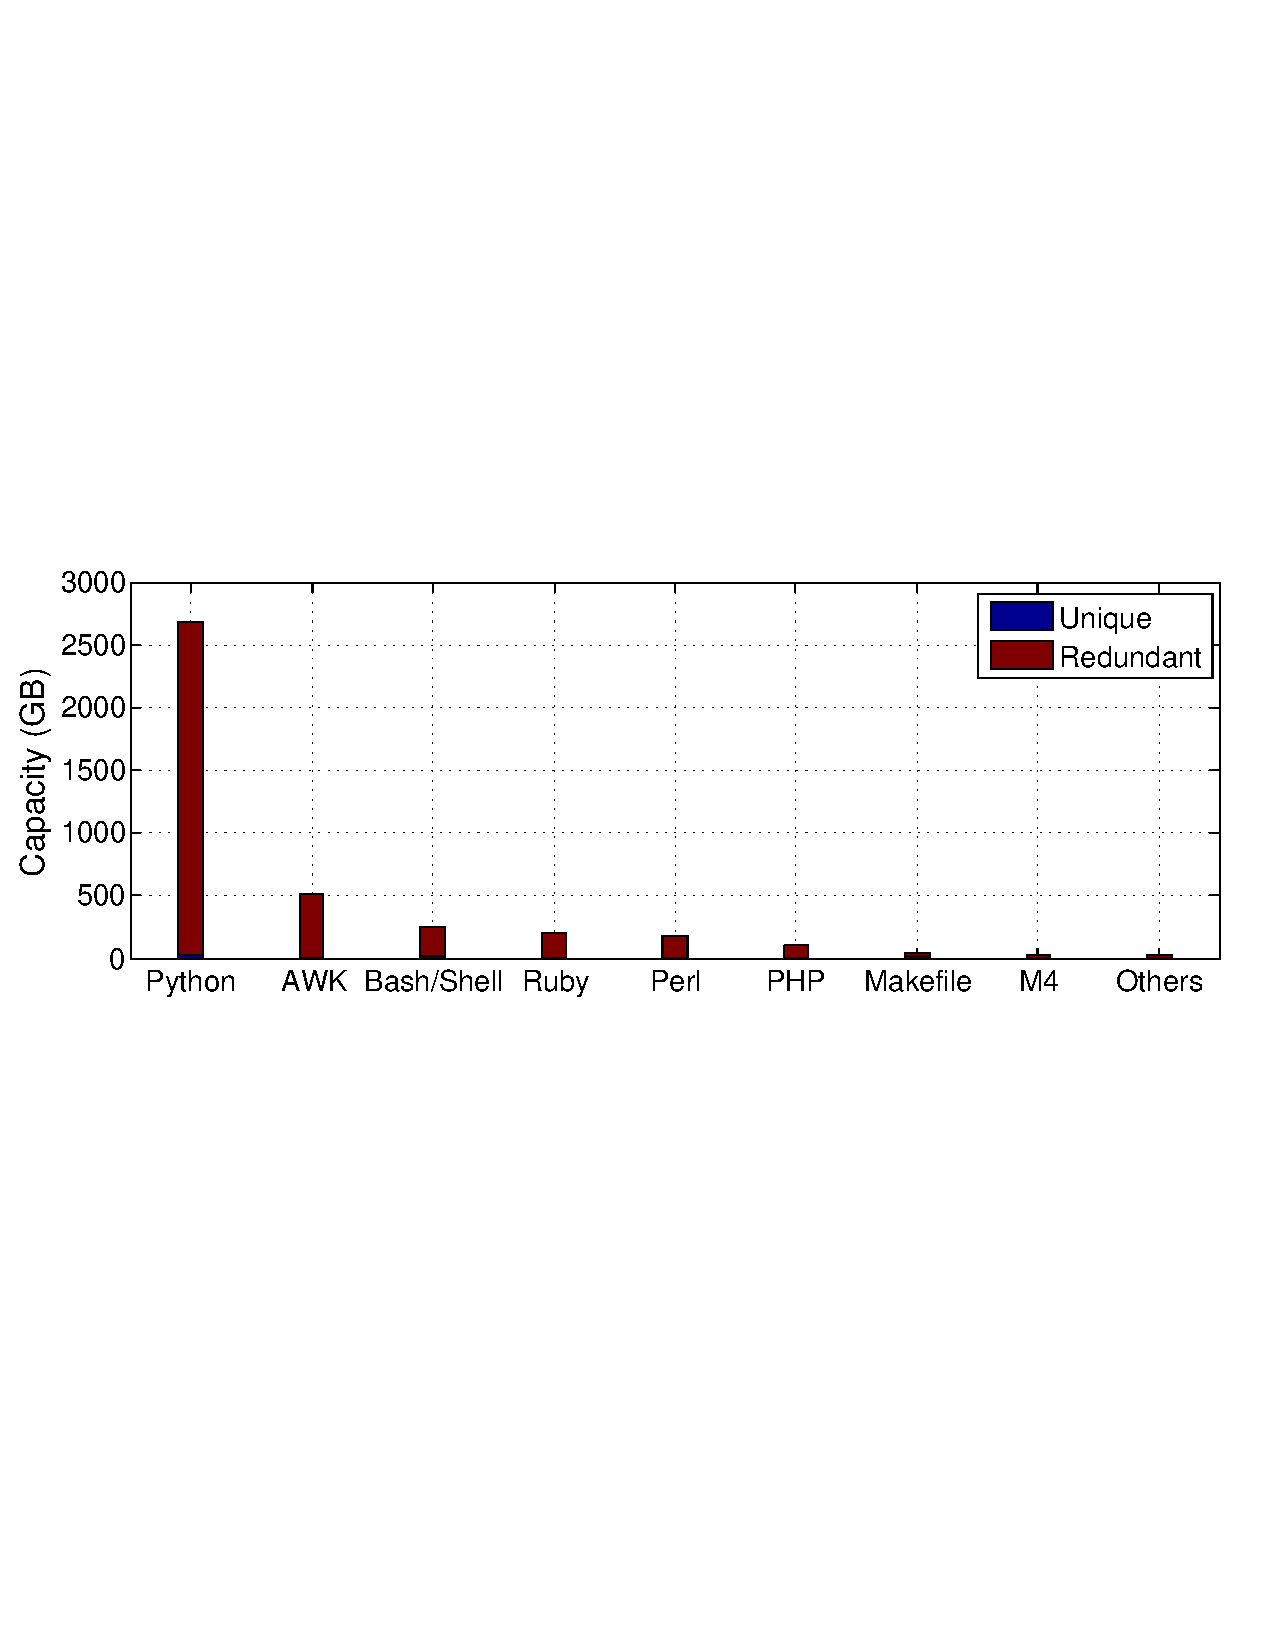
\includegraphics[width=0.5\textwidth]{graphs/type-script-cap}
	\caption{Redundant data vs. unique data for scripts.
	}
	\label{fig:type-script}
\end{figure}

Figure~\ref{fig:type-script} shows the redundant scripts distribution. Python script has the largest number of redundant scripts (238353674, 53.6\%), which take up to 2.6TB storage space, indicating that users are more prone to replicate Python scripts compare to other scripts. 
%This finding also explains that why python byte compiled files takes the largest proportion of intermediate 

We find that users use different scripts in the images. 
For example, 20\%, 9.7\% and 4.4\% of scripts are bash/shell scripts, ruby scripts, and awk scripts. Other scripts such as perl script (4.2\%), php script(3.9\%), makefile script(1.3\%), and M4 macro processor script(0.7\%) are also used.

\subsection{Documents}
\paragraph{Finding 3: 79.7\%, 5.2\%, and 12.4\% of redundant documents are ASCII text, UTF-8/16 text, and HTML/XML/XHTML, which take up over 11TB, 3.4TB, and 3.9TB redundant storage, indicating that users replicate more ASCII text, UTF-8/16 text, and HTML/XML/XHTML compare to other documents}

\begin{figure}
	\centering
	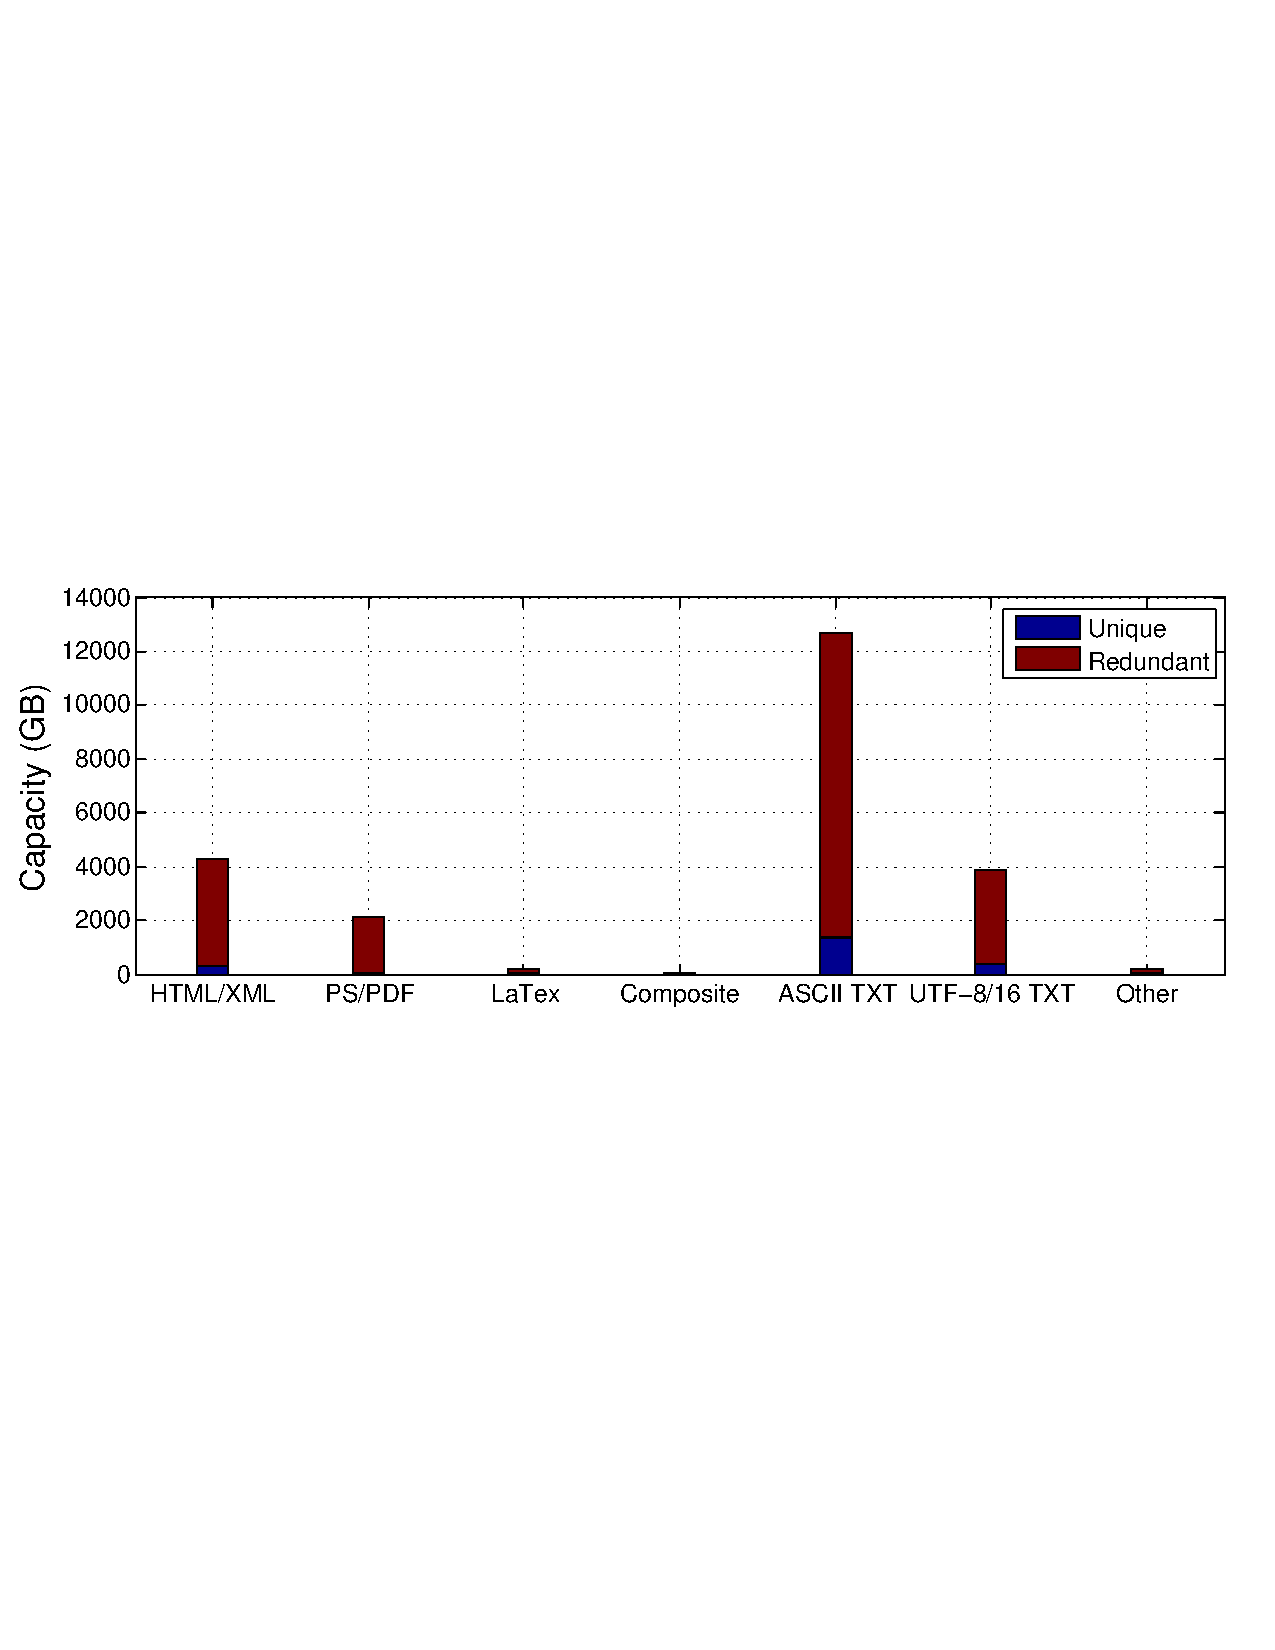
\includegraphics[width=0.5\textwidth]{graphs/type-utili-cap}
	\caption{Redundant data vs. unique data for documents.
	}
	\label{fig:type-doc}
\end{figure}

Figure~\ref{fig:type-doc} presents redundant document distribution. We first group documents into two categories: non-text documents and raw text documents. 
We see that ASCII text files have the largest number of redundant document files (1,758,299,693, 79.7\%), which take up to 11TB storage space, indicating that users replicate more ASCII text. 
12.4\% of the redundant documents are HTML/XML/XHTML documents, which take up to 3.9 TB storage space, indicating users also replicate HTML/XML/XHTML documents in images.  

In addition to ASCII text, 5.2\% of redundant documents are UTF-8/16 unicode text, which take up 3.4 TB storage space.
Various documents are replicated in images, such as PS/PDF documents (0.9\%), LaTex files (1.1\%) and Composite documents (0.01\%)

%79.7\%, 5.2\%, and 12.4\% of redundant documents are ASCII text, UTF-8/16 text, and HTML/XML/XHTML, which take up over 11TB, 3.4TB, and 3.9TB redundant storage, indicating that users replicate more ASCII text, UTF-8/16 text, and HTML/XML/XHTML compare to other documents.
%type-utili-cap
%type-script-cap

\subsection{Database related files}
\paragraph{Finding 4: 28.7\%, 30.9\%, and 11.9\% of redundant database files are Berkeley DB, Mysql, and Dbase related files, which only take up over 1.1 TB, 26 GB, and 47.2 GB redundant storage, indicating that users replicate a lot small database files related to Mysql and Berkeley DB. While there are only 7.3\% of SQLite files, which take up over 2.6TB storage space, indicating SQLite files are much bigger than others}

Figure~\ref{fig:type-db} presents database related redundant files. 30.9\% of redundant database related files are related to MySQL, which only take up to 26GB storage space while SQLite database related redundant files which only take up 7.3\% of redundant database related files consume 2.56 TB storage space, indicating users replicate more MySQL related files and bigger SQLite database related files. %MySQL related files contains mysql table definitation files, mysql misam index files, and mysql misam compressed data. 
Moreover, we also find different redundant database related files are replicated in Docker images. For example, 28.7\%, 11.86\%, and 5.57\% of redundant database files are Berkeley DB, Dbase, and NDBM related files, which take up over 1.1 TB, 47.2 GB, and 7.7 GB redundant storage, indicating that users replicate database files, especially, SQLite and Berkeley DB. 
%While there are only 7.3\% of SQLite files, which take up over 2.6TB storage space, indicating SQLite files are much bigger than others.


\begin{figure*}[t]
	\centering
	\begin{minipage}{0.35\textwidth}
		\centering
		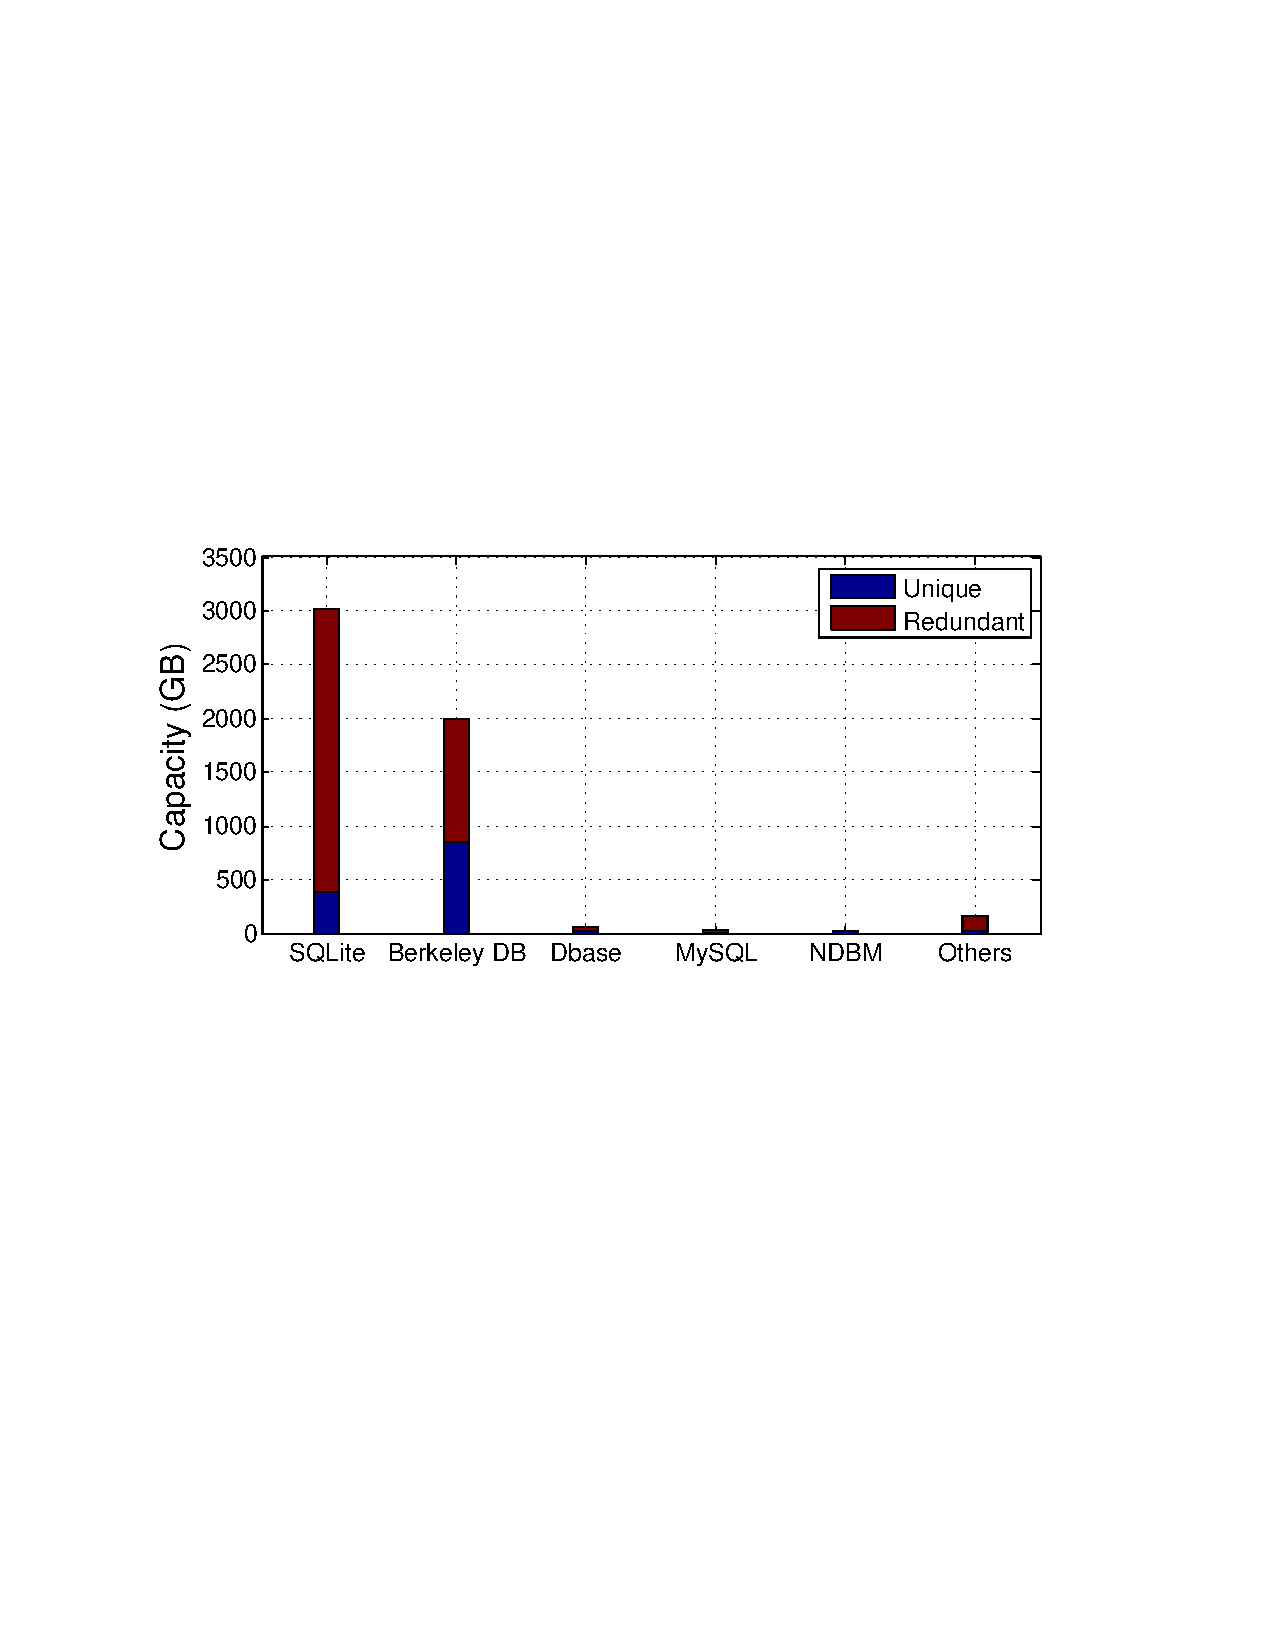
\includegraphics[width=1\textwidth]{graphs/type-db-cap.pdf}
		\caption{Redundant data vs. unique data for database related files}
		\label{fig:type-db}
	\end{minipage}%
	\begin{minipage}{0.278\textwidth}
		\centering
		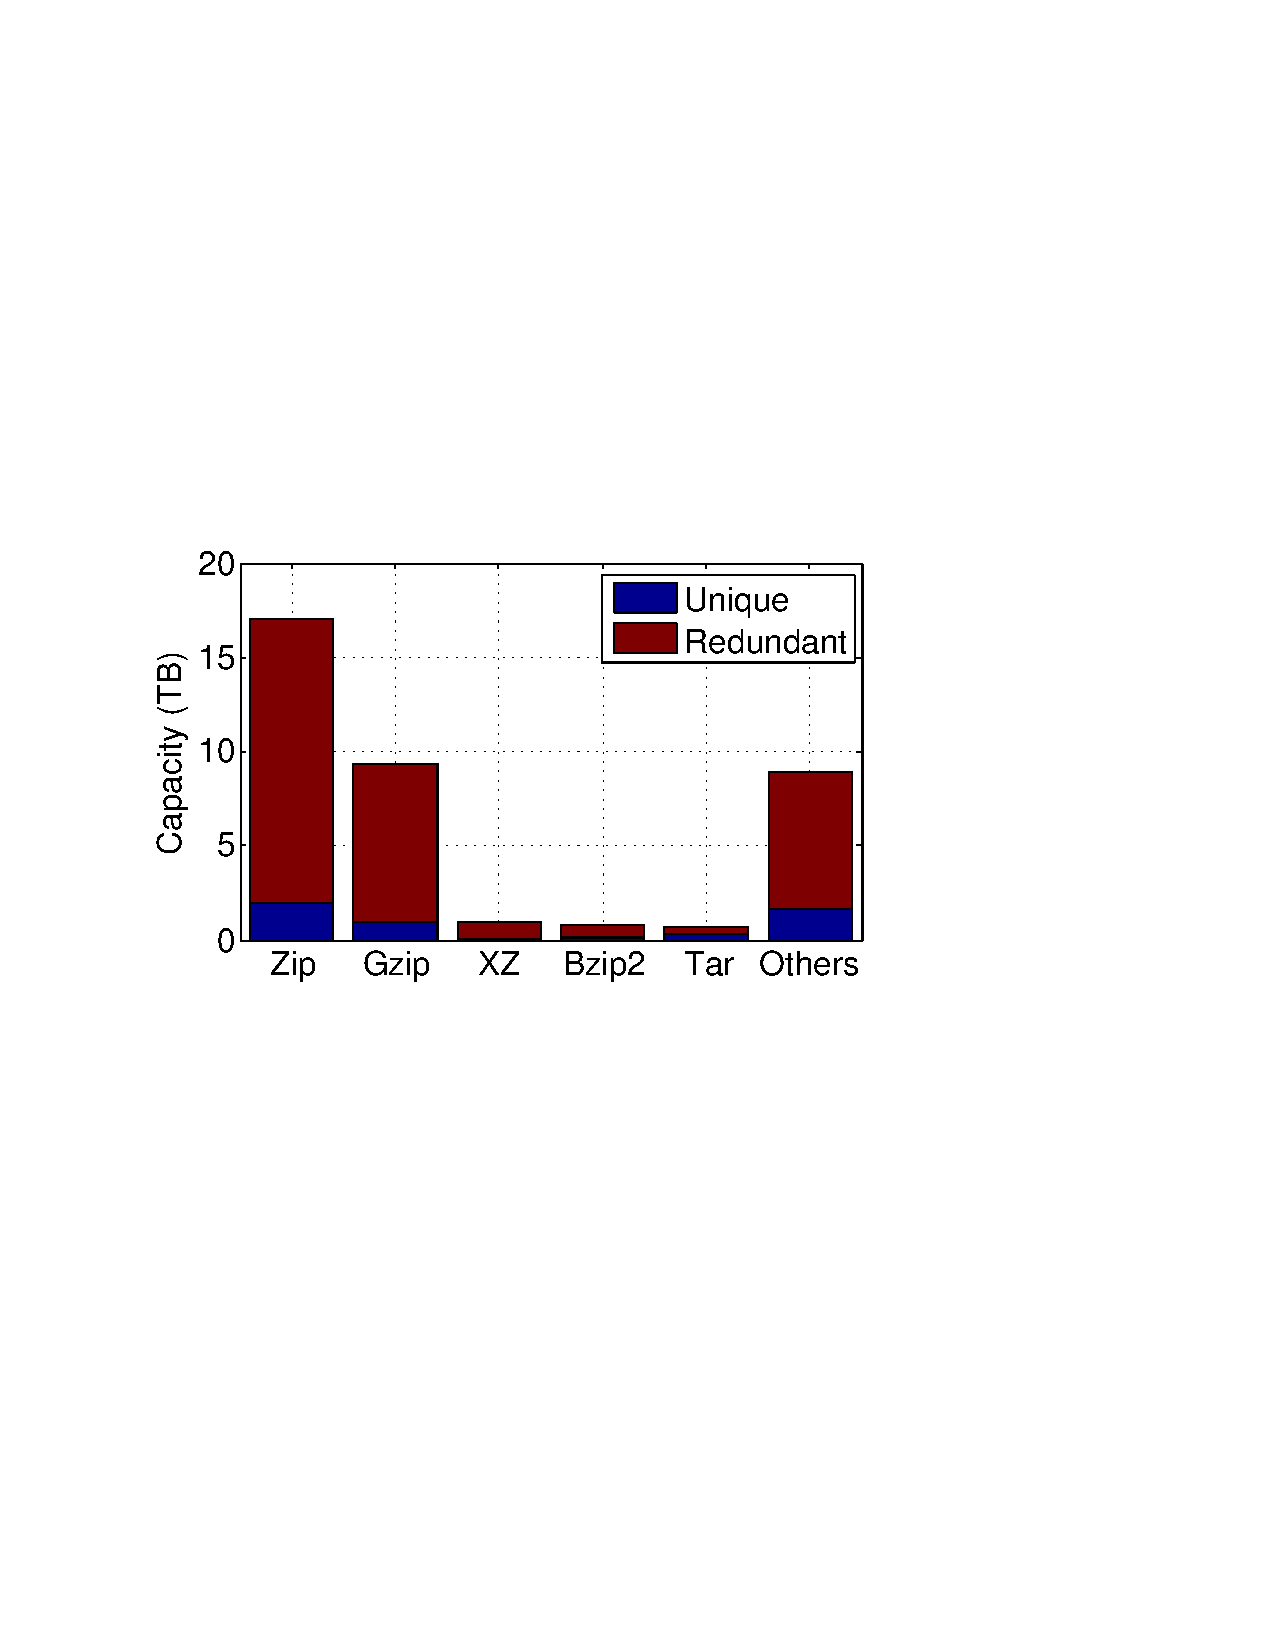
\includegraphics[width=1\textwidth]{graphs/type-tar-type}
		\caption{Redundant data vs. unique data for archival files}
		\label{fig:type-arch}
	\end{minipage}
	\begin{minipage}{0.28\textwidth}
		\centering
		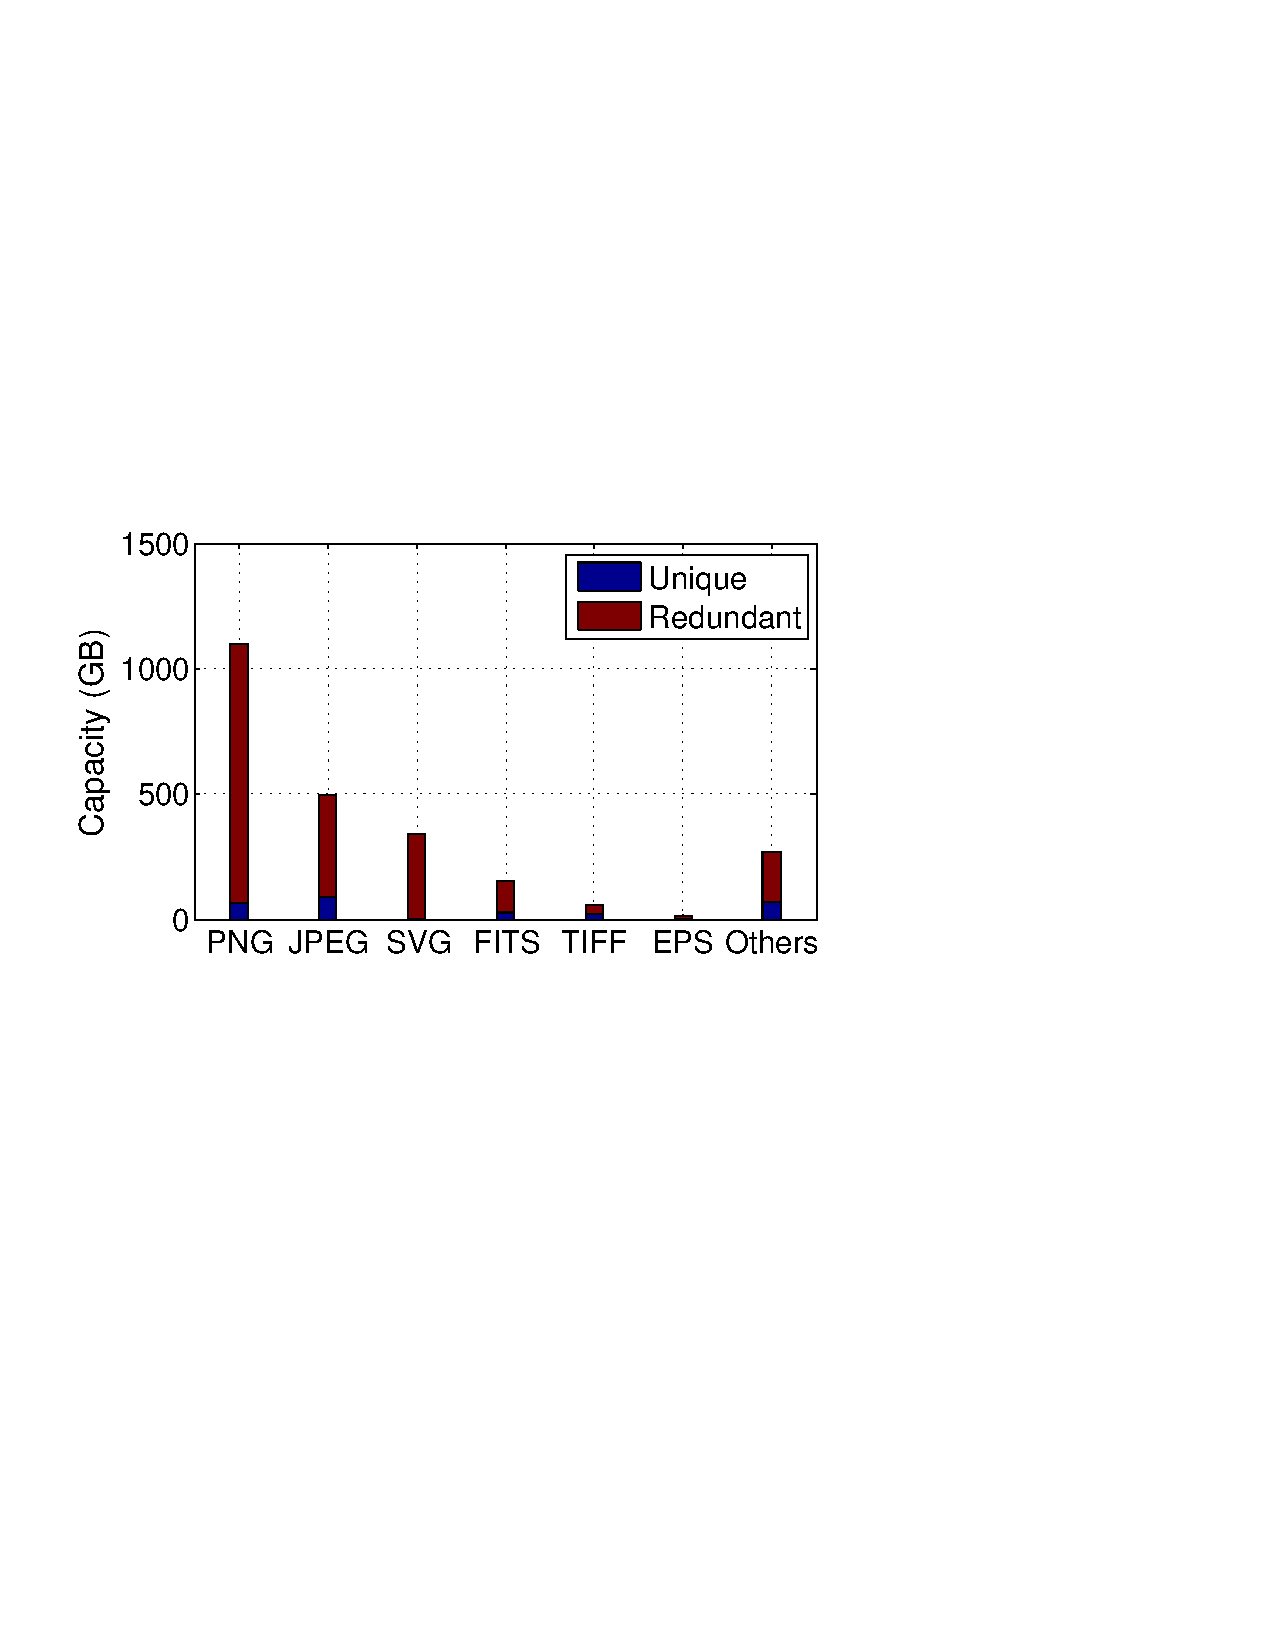
\includegraphics[width=1\textwidth]{graphs/type-image-cap}
		\caption{Redundant data vs. unique data for image files}
		\label{fig:type-img}
	\end{minipage}
\end{figure*}

\subsection{Archival}
\paragraph{Finding 4: 89.5\% and 7.0\% of redundant archival files are Gzip files and Zip files, which take up over 8.4 TB and 15.2 TB storage space, indicating that users replicate more Gzip files and Zip files are much bigger than Gzip files}

Figure~\ref{fig:type-arch} shows the redundant archival file distribution. Gzip files have the largest number of redundant archival files (89.5\%), which take up to 8TB storage space, indicating that users replicate more Gzip compressed files. Although Zip files only take 7.00\% of redundant archival files, they consume 15.5 TB storage space since they are much bigger than Gzip files.

We found other different kinds of archive files, such as XZ (0.42\%), Bzip2(0.96\%), and Tar files(0.36\%).

\subsection{Images}
\paragraph{Finding 4: 67.8\%, 14.3\%, and 4.0\% of redundant image files are PNG, SVG, and JPEG images, which take up over 1.01TB, 4.6 GB, and 401.5 GB storage space, indicating that users also replicate image files, especially, PNG, SVG, and JPEG files}

Figure~\ref{fig:type-img} shows the redundant image file distribution. PNG image files have the largest number of redundant image files (67.8\%), which take up to over 1 TB storage space. 14.3\%, and 4.0\% of redundant image files are SVG, and JPEG images, which take up over 4.6 GB and 401.5 GB storage space, indicating that users also replicate image files, especially, PNG, SVG, and JPEG files. Moreover, there are different redundant image file types, such as FITS (0.05\%), TIFF (0.07\%), and EPS (0.01\%) image files.

%\begin{figure}
%	\centering
%	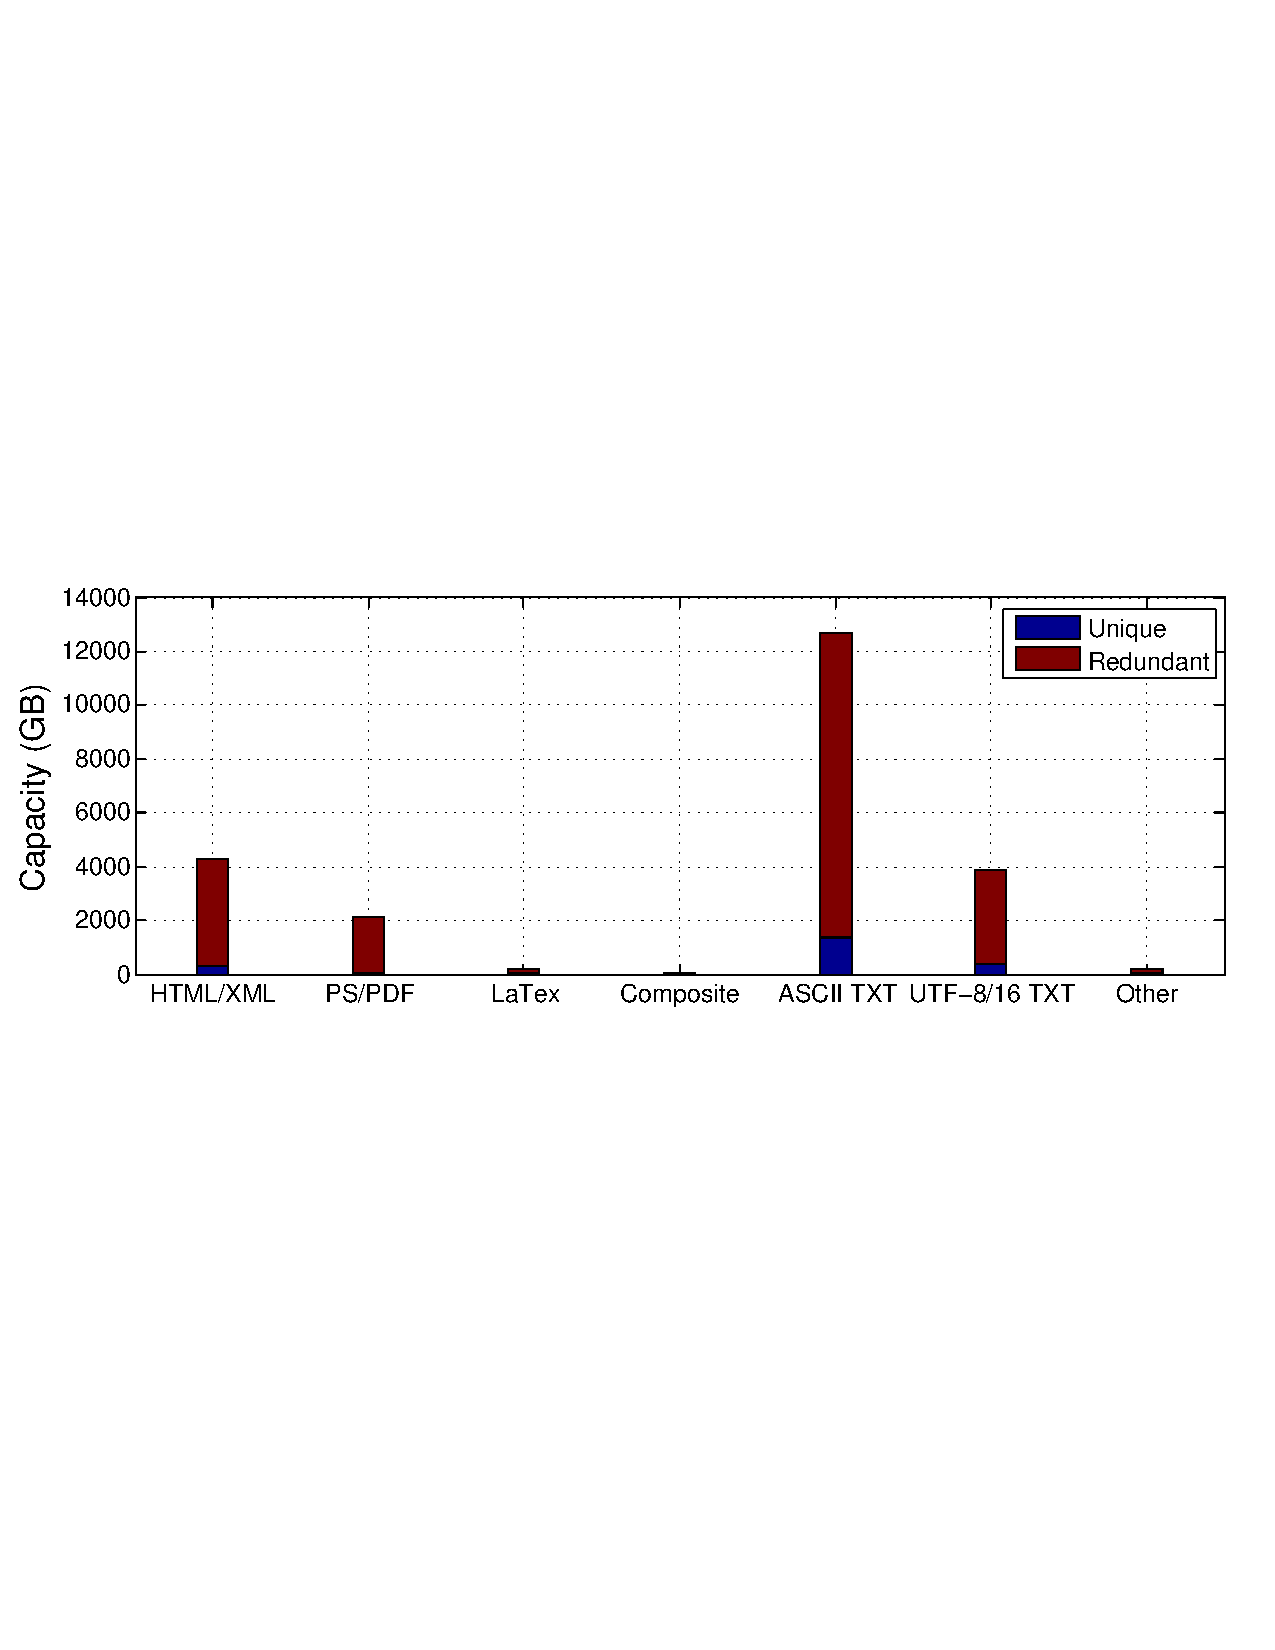
\includegraphics[width=0.35\textwidth]{graphs/type-utili-cap}
%	\caption{Image file distribution.
%	}
%	\label{fig:file_size}
%\end{figure}

%=======================================
%|             OLD VERSION              |
%=======================================

%\begin{table} 
%	\centering 
%	\scriptsize  
%	\caption{Top 20 redundant files' characterization (sorted by repeat cnt.)}
%	\label{tbl:top_dup_files_repeat_cnt} 
%	\begin{tabular}{|l|l|l|l|l|}%p{0.14\textwidth} 
%		\hline 
%		Filename & repeat cnt. & type & extension & size \\
%		\hline
%		&   &   &   &  \\
%		\hline
%		&   &   &   &   \\
%		\hline
%		&   &   &  &    \\
%		\hline
%		&  &  &  & \\
%		\hline
%		& &  &   & \\
%		\hline
%		& &  &   & \\
%		\hline
%		&  &  & & \\
%		\hline
%	\end{tabular} 
%\end{table}

%\begin{table} 
%	\centering 
%	\scriptsize  
%	\caption{Top 20 redundant files' characterization (sorted by capacity)} 
%	\label{tbl:top_dup_files_cap} 
%	\begin{tabular}{|l|l|l|l|l|}%p{0.14\textwidth} 
%		\hline 
%		Filename & repeat cnt. & type & extension & size \\
%		\hline
%		&   &   &   &  \\
%		\hline
%		&   &   &   &   \\
%		\hline
%		&   &   &  &    \\
%		\hline
%		&  &  &  & \\
%		\hline
%		& &  &   & \\
%		\hline
%		& &  &   & \\
%		\hline
%		&  &  & & \\
%		\hline
%	\end{tabular} 
%\end{table}


%\begin{table} 
%	\centering 
%	\scriptsize  
%	\caption{Top redundant file types} 
%	\label{tbl:top_dup_types} 
%	\begin{tabular}{|l|l|l|l|l|l|}%p{0.14\textwidth} 
%		\hline 
%		Type & extension & Num. & size & red. ratio (cnt.)  & red. ratio (cap.)\\
%		\hline
%		&   &   &  & &   \\
%		\hline
%		&   &   &  & &    \\
%		\hline
%		&   &   &   & &   \\
%		\hline
%		&  &  &  & & \\
%		\hline
%		& &  &  & & \\
%		\hline
%		& &  & & &  \\
%		\hline
%		&  &  & & &  \\
%		\hline
%	\end{tabular} 
%\end{table} 

%\subsection{Redundant ratio for directories}
%
%\begin{table} 
%	\centering 
%	\scriptsize  
%	%\begin{minipage}{.5\linewidth}
%	\caption{Inter-dir redundant ratio for dirs in terms of file count and capacity} \label{tbl:intra_dup_ratio_dirs} 
%	\begin{tabular}{|l|l|l|}%p{0.14\textwidth} 
%		\hline 
%		% after \\: \hline or \cline{col1-col2} \cline{col3-col4} ... 
%		% after \\: \hline or \cline{col1-col2} \cline{col3-col4} ... 
%		& File count & Capacity \\
%		\hline
%		Avg. & 98.75\% & 97.33\%\\
%		\hline
%		Median & - & - \\
%		\hline
%		Max. & 1 & 1\\
%		\hline
%		Min.  & 0.87\%  & $<$ 0.00\%\\
%		\hline
%		Stdev.  &  4.70\% & 10.49\\
%		\hline
%		Layer dataset after share.-dedup (Uncompressed) & -  & -\\
%		\hline 
%		Total layer dataset (Uncompressed) &  -	& -\\
%		\hline
%	\end{tabular} 
%\end{table}
%
%\begin{table} 
%	\centering 
%	\scriptsize  
%	%\begin{minipage}{.5\linewidth}
%	\caption{Intra-dir redundant ratio for dirs in terms of file count and capacity} \label{tbl:inter_dup_ratio_dirs} 
%	\begin{tabular}{|l|l|l|}%p{0.14\textwidth} 
%		\hline 
%		% after \\: \hline or \cline{col1-col2} \cline{col3-col4} ... 
%		% after \\: \hline or \cline{col1-col2} \cline{col3-col4} ... 
%		& File count & Capacity \\
%		\hline
%		Avg. & 98.75\% & 97.33\%\\
%		\hline
%		Median & - & - \\
%		\hline
%		Max. & 1 & 1\\
%		\hline
%		Min.  & 0.87\%  & $<$ 0.00\%\\
%		\hline
%		Stdev.  &  4.70\% & 10.49\\
%		\hline
%		Layer dataset after share.-dedup (Uncompressed) & -  & -\\
%		\hline 
%		Total layer dataset (Uncompressed) &  -	& -\\
%		\hline
%	\end{tabular} 
%\end{table}

%\subsection{Redundant directory characterization}
%
%\begin{table} 
%	\centering 
%	\scriptsize  
%	%\begin{minipage}{.5\linewidth}
%	\caption{Top redundant dirs'characterization} 
%	\label{tbl:top_dup_dirs} 
%	\begin{tabular}{|l|l|l|l|}%p{0.14\textwidth} 
%		\hline 
%		% after \\: \hline or \cline{col1-col2} \cline{col3-col4} ... 
%		% after \\: \hline or \cline{col1-col2} \cline{col3-col4} ... 
%		Name & Num. & Redundant ratio & Avg. size \\
%		\hline
%		home &   &   &     \\
%		\hline
%		&   &   &      \\
%		\hline
%		&   &   &      \\
%		\hline
%		&  &  &  \\
%		\hline
%		& &  &   \\
%		\hline
%		& &  &   \\
%		\hline
%		&  &  & \\
%		\hline
%	\end{tabular} 
%\end{table} 

%\begin{figure}
%	\centering
%	\includegraphics[width=0.5\textwidth]{graphs/}
%	\caption{CDF of file repeat count.
%	}
%	\label{fig:file_repeat_count}
%\end{figure}

%\paragraph{Cumulative distribution and probability distribution of file size in terms of unique file size, redundant file size, overall file size}


%\paragraph{Average file size by repeat count}
%
%There is no relation between file repeat count and average file size.
%
%\begin{figure}
%	\centering
%	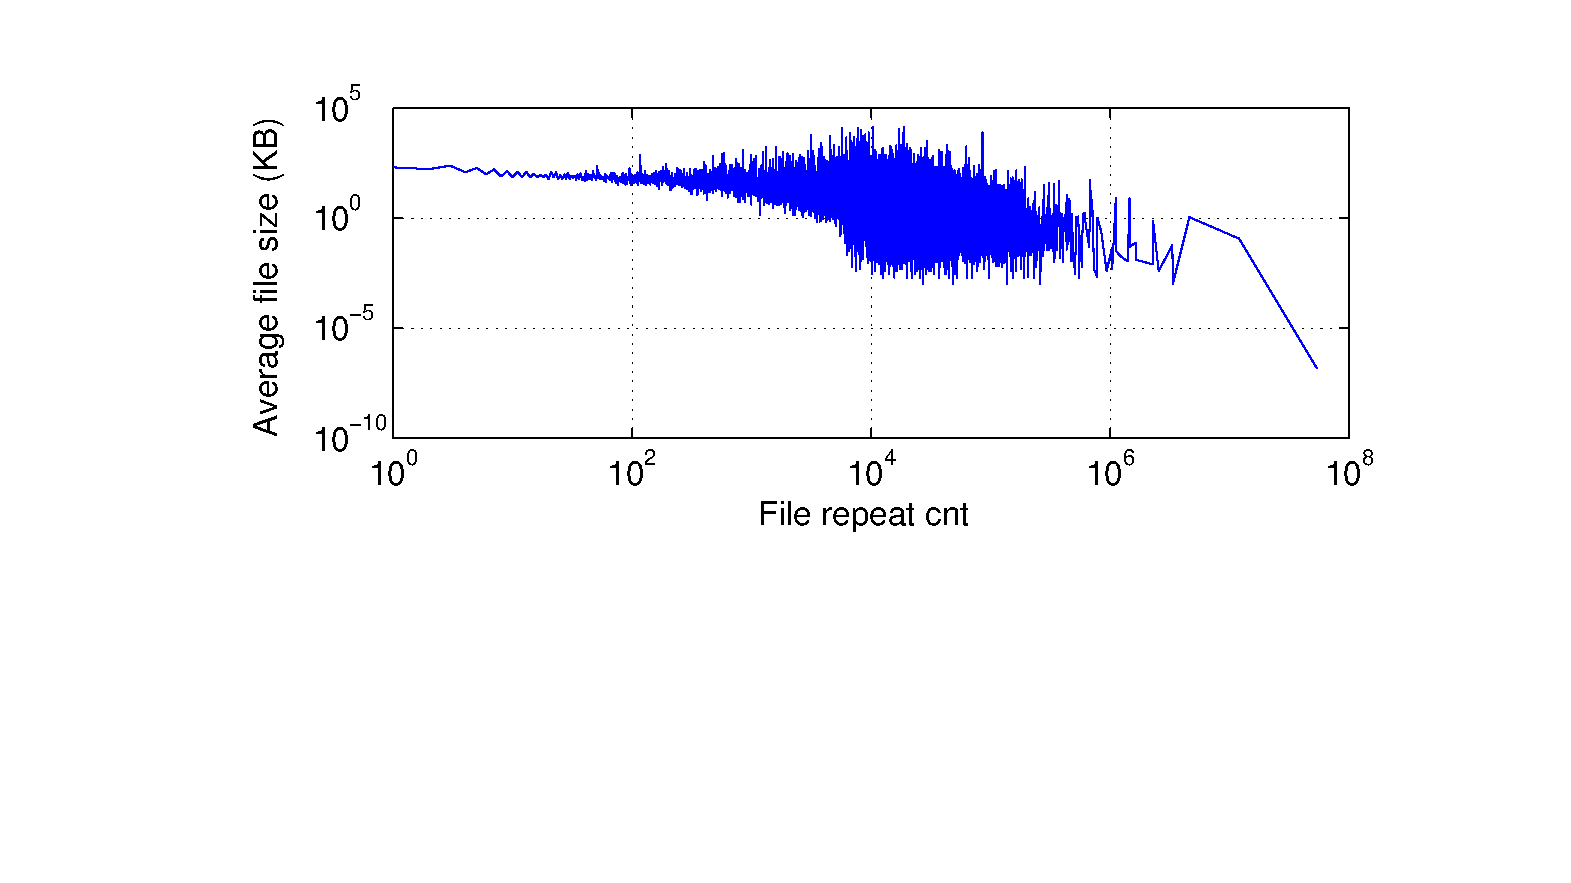
\includegraphics[width=0.5\textwidth]{graphs/avg_size_by_cnt.eps}
%	\caption{Average file size with same repeat count.
%	}
%	\label{fig_avg_size_by_cnt}
%\end{figure}
%
%\paragraph{Redundant ratio by file size for the files with the same content in terms of file count and storage capacity}
%Total size of redundant files with same content(TRS)
%
%97\% of the TRSs are equal or less than 100MB.
%
%\begin{figure}
%	\centering
%	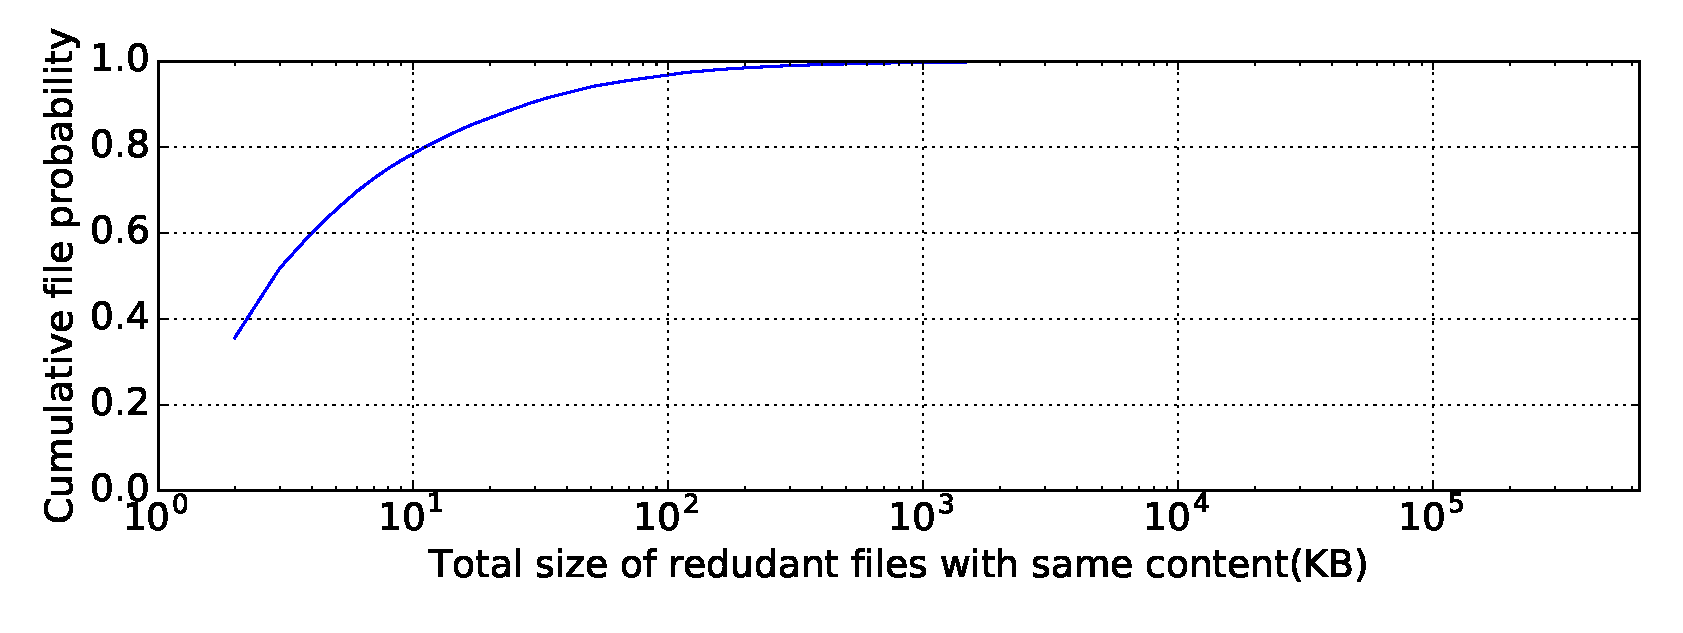
\includegraphics[width=0.5\textwidth]{graphs/Total_size_of_redudant_files_with_same_content-KB.eps}
%	\caption{CDF of total file size with same file content (MB).
%	}
%	\label{fig_total_redundant_same_digest}
%\end{figure}
%
%\paragraph{Redundant ratio by repeat count for the files with the same repeat count in terms of file count and storage capacity}
%
%However, with the increase of file repeat count, the sum of file size with same repeat count becomes smaller.
%
%\begin{figure}
%	\centering
%	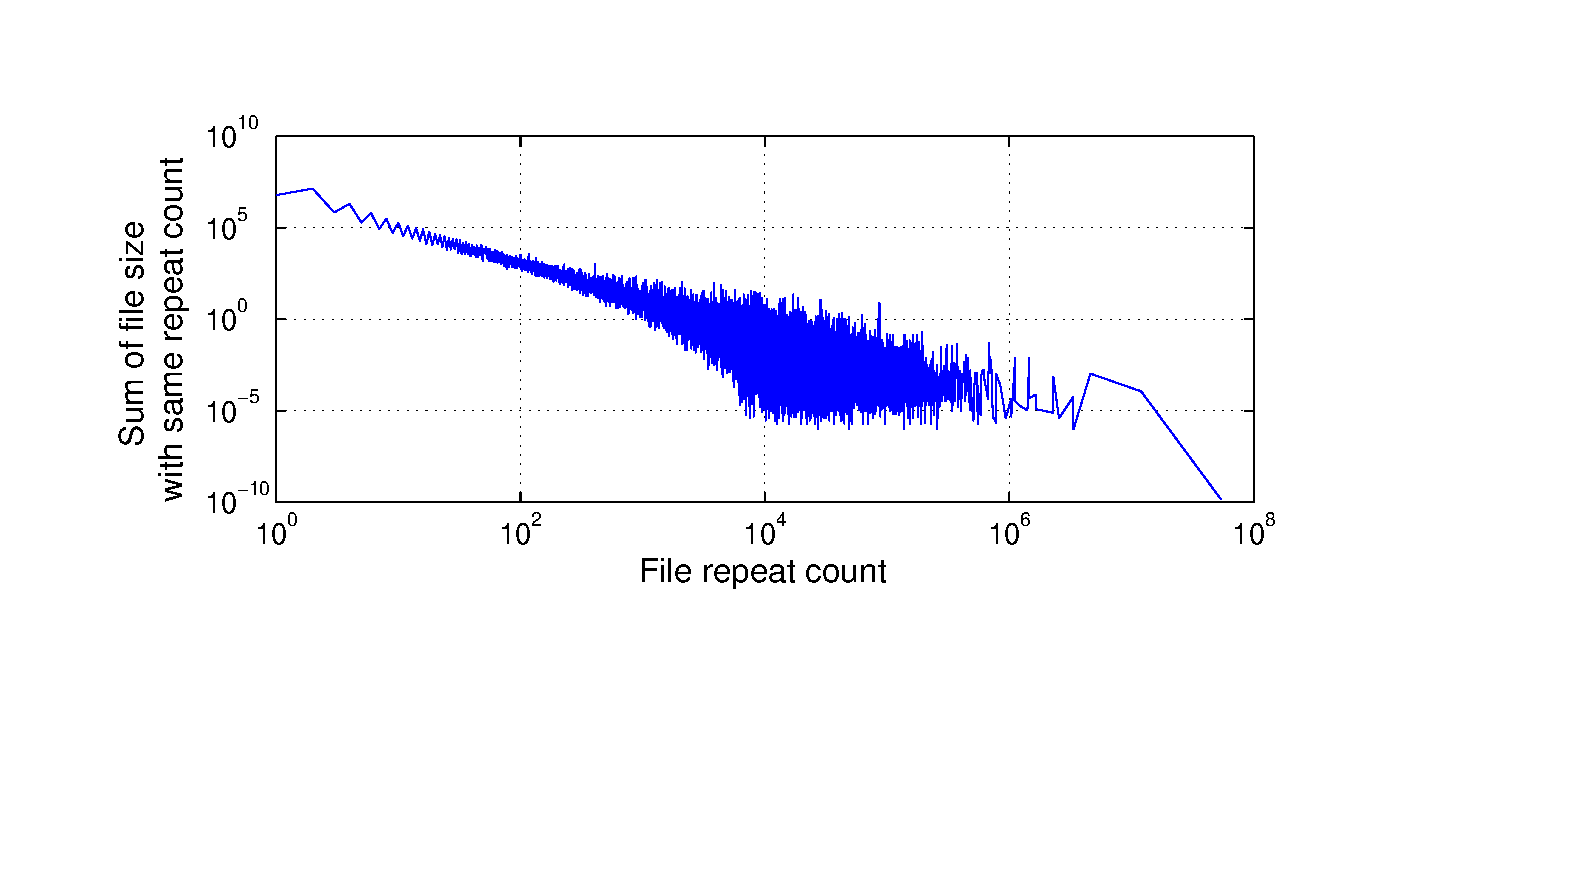
\includegraphics[width=0.5\textwidth]{graphs/sum_size_by_cnt.eps}
%	\caption{Sum of file size with same repeat count.
%	}
%	\label{fig_sum_by_cnt}
%\end{figure}

%
%\paragraph{Cumulative distribution and probability distribution of file repeat count}
%\begin{table} 
%	\centering 
%	\scriptsize  
%	%\begin{minipage}{.5\linewidth}
%	\caption{Summary of image types} \label{tbl:redundant_ratio} 
%	\begin{tabular}{|l|l|l|}%p{0.14\textwidth} 
%		\hline 
%		% after \\: \hline or \cline{col1-col2} \cline{col3-col4} ... 
%		% after \\: \hline or \cline{col1-col2} \cline{col3-col4} ... 
%		Image types & num. & avg. redundant ratio  \\
%		\hline
%		  &   &        \\
%		\hline
%		  &   &         \\
%		\hline
%		   &   &       \\
%		   \hline
%		other     &   &       \\
%		\hline
%	\end{tabular} 
%\end{table}

%\subsection{Redundant files with same filename and relative path}
%
%\subsection{Common directories that contains redundant files}
%
%\subsection{Redundant tar files}
%\begin{table} 
%	\centering 
%	\scriptsize  
%	%\begin{minipage}{.5\linewidth}
%	\caption{Summary of file \& dir. characterization} \label{tbl:sum_file_dir_char} 
%	\begin{tabular}{|l|l|l|l|l|}%p{0.14\textwidth} 
%		\hline 
%		% after \\: \hline or \cline{col1-col2} \cline{col3-col4} ... 
%		% after \\: \hline or \cline{col1-col2} \cline{col3-col4} ... 
%		Metrics & max & min & median & avg.\\
%		\hline
%		File size &   &   &   &  \\
%		\hline
%		File size (repeat cnt. $>$ 1) &   &   &    &  \\
%		\hline
%		File size (repeat cnt. $=$ 1) &   &   &    &  \\
%		\hline
%		\hline
%		Dir. size &  &  & & \\
%		\hline
%		File cnt. per dir & &  &  & \\
%		\hline
%		Redundant ratio & &  &  & \\
%		\hline
%		Dir. depth  &  &  & & \\
%		\hline
%	\end{tabular} 
%\end{table} 